\chapter{Classical Bayesian Decision Analysis} % Main chapter title

\label{chapter2} % For referencing the chapter elsewhere, use \ref{Chapter1} 

\lhead{Chapter 2. \emph{Classic Bayesian Decision Analysis}}

In the introduction we discussed the use of Bayesian reasoning and modelling techniques at the inception of probabilistic ESs. Although we noted the inappropriateness of standard methodologies for the needs of current applications, several systems are still based on these traditional models. The theory we develop in the following chapters is a generalisation of Bayesian methodologies and models to formally accommodate the beliefs of different group of experts. We need therefore first to provide a broad overview of the currently available Bayesian modelling tools for DMs. 

The chapter is structured as follows. In Section \ref{sec:bayesianreasoning} we outline the Bayesian formalism of inference. Section \ref{sec:SEU} introduces the Subjective Expected Utility (SEU) methodology which embeds canons of rational decision making and defines rules to make decisions that are optimal according to these canons. The SEU model basically consists of two main ingredients: a probability function, representing the beliefs of a DM, and a utility function, representing her values. Sections \ref{sec:prob} and  \ref{sec:ut} introduce methodologies to represent respectively probability and utility functions in a multivariate setting. In such a case the definition and elicitation of these functions is often prohibitive. Independence concepts have been introduced to factorise these into subfunctions with a smaller number of arguments. Such factorisations can  often be depicted by a graph providing a powerful and intuitive representation of the relationships between the elements of the problem. Therefore our discussion is mainly based on graphical models, for both probabilities and utilities. We introduce here a new subclass of certain utility graphical models defined in \citet{Abbas2010} that have interesting properties in the domains we address in this thesis \citep[see also][]{Leonelli2015}.

In Section \ref{sec:dec} we introduce classes of models that explicitly represent both probabilities and utilities, and the decisions available to a single DM. Again our discussion focuses on graphical models and in particular on the Influence Diagram (ID) model. We consider in this thesis the models class of multiplicative IDs defined in \citet{Leonelli2015a} and introduce a new fast evaluation algorithm for these models.

The SEU model is only capable of representing how a single DM should rationally commit to decisions. However, as we have seen in Chapter \ref{chapter1}, policy choices are seldom made by just one person. There might be several DMs sharing the authority and responsibility of choosing a certain policy, many stakeholders who are affected by the DM's decision, and experts that are consulted by the DMs. In Section \ref{sec:group} we briefly review the literature on both group decision making and the use of expert judgement to support decision making. We then conclude with a more detailed explanation of the contributions of this thesis and a discussion.

\section{Bayesian Reasoning}
\label{sec:bayesianreasoning}
\subsection{The Full Probabilistic Case}
A problem domain is denoted by an often large dimensional random vector $\bm{Y}$ with sample space $\bm{\mathcal{Y}}$. We denote by $\bm{y}$ a generic instantiation of $\bm{Y}$ and we let $\bm{\theta}\in\bm{\Theta}$ parametrise the density function $f$ of $\bm{Y}$. In a Bayesian framework the parameter $\bm{\theta}$ is itself a random variable. We let $\pi$ denote its density function. For the purpose of this section, the vectors are assumed to be continuous.\footnote{In discrete domains integrals are simply substituted by summations. We denote probability mass functions by $p$.}  Let $\bm{X}$ be a random vector sampled from the same population as $\bm{Y}$ providing some data points $\bm{x}$. Within this framework, \textbf{Bayes theorem} can be  simply  employed to update the beliefs about $\bm{\theta}$ after evidence $\bm{x}$ has been observed as 
\begin{equation}
\label{eq:bayes}
\pi(\bm{\theta}\;|\;\bm{x})=\frac{f(\bm{x}\;|\;\bm{\theta})\pi(\bm{\theta})}{f(\bm{x})}=\frac{f(\bm{x}\;|\;\bm{\theta})\pi(\bm{\theta})}{\int_{\bm{\Theta}}f(\bm{x}\;|\;\bm{\theta})\pi(\bm{\theta})\dr \bm{\theta}}.
\end{equation}
The terms of equation (\ref{eq:bayes}) have all a meaning. The so called \textit{prior distribution}, $\pi(\bm{\theta})$, represents the beliefs of the DM about the parameter $\bm{\theta}$ before evidence $\bm{x}$ is introduced into the system. If for example $\bm{Y}$ were a univariate binary random variable, then $\pi(\bm{\theta})$ would simply be a probability distribution over $[0,1]$ representing the beliefs of the DM about the probability of a success (for simplicity here we have chosen a discrete example). Although we do not further discuss these issues, we note that there is now an extensive literature and several software that allow for a faithful elicitation of such prior beliefs \citep[see e.g.][]{O'Hagan2006a}. The other term at the numerator, $f(\bm{x}\;|\;\bm{\theta})$, is usually called a \textit{likelihood function}. In a Bayesian setting this measures the DM's degree of belief in the data taking certain values given that the parameter is fixed to a certain hypothetical value. Continuing the example above, the likelihood would be in this situation the density of a Bernoulli random variable with a hypothetical unknown probability of success. The denominator of equation (\ref{eq:bayes}), $f(\bm{x})$,  simply corresponds to a normalising constant, since for a Bayesian all the relevant information is related to $\bm{\theta}$. Therefore, equation (\ref{eq:bayes}) is often presented in the following form,
\begin{equation}
\label{eq:proprbayes}
\pi(\bm{\theta}\;|\;\bm{x})\propto f(\bm{x}\;|\;\bm{\theta})\pi(\bm{\theta}),
\end{equation}
where $\propto$ corresponds to proportionality.  The corresponding normalising constant is often difficult to compute, since it requires an integration over an arbitrarily large space. Thus, equation (\ref{eq:proprbayes}) often represents a computationally less intensive version of equation (\ref{eq:bayes}). Finally, the \textit{posterior} distribution, $\pi(\bm{\theta}\;|\;\bm{x})$, is simply the revised density function of $\bm{\theta}$ after  evidence $\bm{x}$ has been observed. Suppose, for instance, that $\bm{x}$ in the running example is the result of ten coin tosses showing all head (or 1) and assume that the prior distribution was symmetric around 1/2. The posterior distribution would then be left-skewed and values in the interval $(1/2,1]$ would have in general higher probability than the ones in $[0,1/2]$. Henceforth, we assume all these densities to represent the subjective Bayesian beliefs of a DM \citep[for more details on the various interpretation of probabilities and the adequateness of the Bayesian interpretation in decision making, see e.g.][]{O'Hagan2004a,French2000b}.

Depending on whether the variables are continuous or discrete, on their support and  on the domain under study, there exist many different possible choices for both the likelihood function and the prior density. We review a variety of standard models in Appendix \ref{appendixE}, as for example the Bayesian Normal linear model, which assumes a Normal distribution for both the likelihood and the prior density of the mean when the variance is assumed to be known. We note here that a computationally efficient choice of prior and likelihood are of two that are \textit{conjugate} \citep{Bernardo2009, O'Hagan2004a}. This is the case whenever the posterior, computed via Bayes theorem, lies in the same family of distributions as the prior. In the example above, if $\pi(\bm{\theta})$ were chosen to follow a Beta distribution with parameters $(a,b)\in\mathbb{R}^2_{>0}$, then the posterior would also be a Beta with some new parameters $(a',b')\in\mathbb{R}^2_{>0}$ (see Appendix \ref{sec:beta}).

Implicitly in equation (\ref{eq:bayes}) we assumed that the parameters of the distribution of $\bm{\theta}$ were known. Within the Bayesian approach this does not necessarily have to be  the case and several different levels or layers of uncertainty can be introduced. This modelling strategy is usually referred to as multilevel or \textit{hierarchical modelling} \citep{Gelman2006}. For example, the parameters of the Beta distribution above, $a$ and $b$, could have been assumed to be random and depending on some other parameters, which could have further been random variables, and so forth. For the purpose of this thesis, we only consider hierarchies consisting of one layer so that the parameters of $\pi(\bm{\theta})$ are known. These are usually referred to as \textit{hyperparameters}. 

\subsection{Moments}
Density functions can be easily summarised using the notion of \textit{moments}, which can describe some of their features. Moments are expected values of power functions of random variables. To introduce these, we first define the concept of expected  values. Let $g:\bm{\mathcal{Y}}\rightarrow \bm{\mathcal{Y}}'$, i.e. $g$ is a function mapping elements of $\bm{\mathcal{Y}}$ into $\bm{\mathcal{Y}}'$. 

\begin{definition}
\label{def:expectedvalue}
The expected value of $g(\bm{Y})$ is defined as\footnote{In the discrete case equations (\ref{eq:exp}) and (\ref{eq:condexp}) have a slightly different form which is not relevant for this thesis and can be found in \citet{Casella2002}.}
\begin{equation}
\label{eq:exp}
\E(g(\bm{Y}))=\int_{\bm{\mathcal{Y}}'}g(\bm{y})f(\bm{y})\dr \bm{y}=\int_{\bm{\Theta}}\E(g(\bm{Y})\;|\;\bm{\theta})\pi(\bm{\theta})\dr \bm{\theta},
\end{equation}
where the expected value $\E(g(\bm{Y})\;|\;\bm{\theta})$ conditional  on $\bm{\theta}$ is defined as
\begin{equation}
\label{eq:condexp}
\E(g(\bm{Y})\;|\;\bm{\theta})=\int_{\bm{\mathcal{Y}}'}g(\bm{y})f(\bm{y}\;|\;\bm{\theta})\dr\bm{y}.
\end{equation}
\end{definition}
For continuity with the previous section, we considered in Definition \ref{def:expectedvalue} quantities conditional on the parameter vector $\bm{\theta}$. However, in general, the conditioning might operate over any random vector of interest.

We can now define the notion of moment. Let, for $n\in\mathbb{Z}_{\geq 1}$, $[n]=\{1,\dots,n\}$, $\bm{s}^\T=(s_1,\dots,s_n)=(s_i)_{i\in[n]}\in \mathbb{Z}_{\geq 0}^n$ and $\bm{Y}^{\bm{s}}=Y_1^{s_1}\cdots Y_n^{s_n}$. 

\begin{definition}
We say that the moment of \emph{order} $\bm{s}$ of $\bm{Y}$ is $\E\left(\bm{Y}^{\bm{s}}\right)$. The moment of order $\bm{s}$ of $\bm{Y}$ conditional on $\bm{\theta}$ is $\E\left(\bm{Y}^{\bm{s}}\;|\;\bm{\theta}\right)$. 
\end{definition}

 We now define some specific moments.

\begin{definition}
Let $\bm{Y}$, $\bm{Y}_i$ and $\bm{Y}_j$ be  random vectors of dimension $n$. The \emph{expectation} of $\bm{Y}$ is $\E(\bm{Y})=\E(\bm{Y}^{\bm{1}})$,  where $\bm{1}$ is a vector of dimension $n$ with $1$ in each entry, whilst the \emph{variance} of $\bm{Y}$, $\V(\bm{Y})$, is $\E((\bm{Y}-\E(\bm{Y}))(\bm{Y}-\E(\bm{Y}))^\T)$. The \emph{covariance} between $\bm{Y}_i$ and $\bm{Y}_j$, $\Cov(\bm{Y}_i,\bm{Y}_j)$, is $\E((\bm{Y}_i-\E(\bm{Y}_i))(\bm{Y}_j-\E(\bm{Y}_j))^\T)$. 
\end{definition}

\begin{definition}
Let $\bm{Y}$, $\bm{Y}_i$ and $\bm{Y}_j$ be  random vectors of dimension $n$. The \emph{conditional expectation} of $\bm{Y}$ given $\bm{\theta}$ is $\E(\bm{Y}\;|\;\bm{\theta})=\E(\bm{Y}^{\bm{1}}\;|\;\bm{\theta})$, whilst the \emph{conditional variance} of $\bm{Y}$ given $\bm{\theta}$, $\V\left(\bm{Y}\;|\;\bm{\theta}\right)$, is $\E\left(\left(\bm{Y}-\E(\bm{Y}\;|\;\bm{\theta})\right)(\bm{Y}-\E(\bm{Y}\;|\;\bm{\theta})\right)^\T\;|\;\bm{\theta})$. The \emph{ conditional covariance} between $\bm{Y}_i$ and $\bm{Y}_j$ given $\bm{\theta}$, $\Cov(\bm{Y}_i,\bm{Y}_j\;|\;\bm{\theta})$, is $\E((\bm{Y}_i-\E(\bm{Y}_i\;|\;\bm{\theta}))(\bm{Y}_j-\E(\bm{Y}_j\;|\;\bm{\theta}))^\T\;|\;\bm{\theta})$.
\end{definition}
We now list some properties of these operators \citep[see e.g.][]{Casella2002}.
\begin{proposition}
\label{prop:propmom}
Let $\bm{Y}_i$ and $\bm{Y}_j$ be random vectors of dimension $n$. Further let $B_i$ and $B_j$ be $n\times n$ matrices with real entries, whilst $\bm{b}\in\mathbb{R}^n$. The following identities hold. 
\begin{align}
\E(B_i\bm{Y}_i\pm B_j\bm{Y}_j\pm \bm{b}\;|\;\bm{\theta})&=B_i\E(\bm{Y}_i\;|\;\bm{\theta})\pm B_j\E(\bm{Y}_j\;|\;\bm{\theta}) \pm \bm{b},\nonumber\\
\Cov(\bm{Y}_i,\bm{Y}_j\;|\;\bm{\theta})&=\E\left(\bm{Y}_i\bm{Y}_j^\T\;|\;\bm{\theta}\right)-\E(\bm{Y}_i\;|\;\bm{\theta})\E(\bm{Y}_j\;|\;\bm{\theta})^\T,\nonumber\\
\V(B_i\bm{Y}_i \pm B_j\bm{Y}_j\pm \bm{b}\;|\;\bm{\theta})&=B_i\V(\bm{Y}_i\;|\;\bm{\theta})B_i^\T+B_j\V(\bm{Y}_j\;|\;\bm{\theta})B_j^\T\pm 2B_i\Cov(\bm{Y}_i,\bm{Y}_j\;|\;\bm{\theta})B_j.\nonumber
\end{align}
\end{proposition}

The following proposition then links conditional and unconditional moments of order one and two.

\begin{proposition}
\label{prop:towerrules}
Let $\bm{Y}_i$ and $\bm{Y}_j$ be two random vectors. Then
\begin{align}
\E(\bm{Y}_i)&=\E(\E(\bm{Y}_i\;|\;\bm{\theta})),\label{eq:tower}\\
\V(\bm{Y}_i)&=\E(\V(\bm{Y}_i\;|\;\bm{\theta}))+\V(\E(\bm{Y}_i\;|\;\bm{\theta})).\label{eq:totalvariance}
\end{align}
\end{proposition}
Equations (\ref{eq:tower}) and (\ref{eq:totalvariance}) are usually called \textit{tower rules} of moments. Specifically, equation (\ref{eq:tower}) is the tower rule of expectations, whilst equations (\ref{eq:totalvariance}) is referred to as \textit{law of total variance}.
 \citet{Brillinger1969} generalised the identities (\ref{eq:tower})-(\ref{eq:totalvariance}) and deduced a recursive formula to compute cumulants of any finite order. Cumulants can be thought of as a function of the moments, and vice versa. Many properties of random vectors can be more easily investigated using cumulants than moments \citep[see e.g.][]{Zwiernik2012}.

\section{The Subjective Expected Utility Model}
\label{sec:SEU}
In the previous section we introduced the Bayesian framework for reasoning about and modelling uncertainty. However, the Bayesian approach further provides an axiomatic basis for decision making, which embodies canons of rationality, usually referred to as the \textbf{SEU} model. Broadly speaking this consists of three main components:
\begin{itemize}
\item a decision space $\bm{\De}$ which includes the decisions $\bm{d}\in\bm{\De}$ available to the DM;
\item a probability density $f$ over the unknown state $\y\in \bm{\MY}$ of a vector of relevant random variables $\Y$;
\item a utility function $u(\bm{d},\bm{r}(\y,\bm{d}))$ describing the DM's preferences over some random vector $\bm{R}$, whose instantiation $\bm{r}=\bm{r}(\y,\bm{d})$ is a function of both $\bm{d}$ and $\y$, and takes values in $\bm{\Rs}$.
\end{itemize}

Having dealt with probability in Section \ref{sec:bayesianreasoning}, we now focus on utility functions.
\begin{definition}
\label{def:ut}
A utility function with arguments $\bm{d}$ and $\bm{r}$ is a real-valued function unique up to increasing affine transformations, $u:\bm{\De}\bigtimes\bm{\Rs}\rightarrow \mathbb{R}$, such that 
\begin{equation*}
\label{eq:utility}
\forall \; (\bm{d}_i,\bm{r}_i), (\bm{d}_j,\bm{r}_j)\in \bm{\De}\bigtimes\bm{\Rs},\;\; u(\bm{d}_i,\bm{r}_i)\geq u(\bm{d}_j,\bm{r}_j) \Leftrightarrow (\bm{d}_i,\bm{r}_i) \succeq (\bm{d}_j,\bm{r}_j),
\end{equation*}
where  $(\bm{d}_i,\bm{r}_i) \succeq (\bm{d}_j,\bm{r}_j)$ means that the DM finds that $(\bm{d}_i,\bm{r}_i)$ is at least as preferable as $(\bm{d}_j,\bm{r}_j)$. The $\bigtimes$ denotes the Cartesian product.
\end{definition}
Note that in general utility functions only represent preference rankings and do not include any representation of the strength of these preferences. Formally, utilities are only unique up to increasing affine transformations. Therefore, utility functions are usually normalised so that they take values between 0 and 1, i.e. $u:\bm{\De}\bigtimes\bm{\Rs}\rightarrow [0,1]$. There have been some theoretical studies considering strength of preferences \citep[see e.g.][]{Argyris2014}, but these are not considered in this thesis. 

The study of utility functions dates back to the work of \citet{VonNeumann2007} which mostly concerned the theory of games. Throughout the following years, several different authors derived different constructions of the SEU model based on different, but related, sets of axioms \citep[e.g.][]{Anscombe1963,DeGroot2005,Savage1972}.  We assume throughout the thesis that a set of axioms underpinning the SEU model holds and that the DM is able to elicit both a utility function and a probability distribution respecting one of these.

Now that utility functions have been introduced, we can show how the SEU model combines probabilities and utilities to guide decision making. Decisions are ranked according to their associated expected utility.

\begin{definition}
Let $\bm{\mathcal{D}}$ be a decision space, $f$ a density function for a random vector $\bm{Y}$ parametrised by $\bm{\theta}$ and $u$ a utility function with arguments $\bm{d}\in \bm{\mathcal{D}}$ and $\bm{r}=\bm{r}(\bm{y},\bm{d})$. The \textbf{expected utility} of a decision $\bm{d}$, $\bar{u}(\bm{d})$, is defined as
\begin{align}
\label{eq:expectedut}
\bar{u}(\bm{d})=&\int_{\bm{\Theta}}\bar{u}(\bm{d}\;|\;\bm{\theta})\pi(\bm{\theta}\;|\;\bm{d})\dr \bm{\theta},\\
\intertext{where}
\label{eq:expectedcondut}
\bar{u}(\bm{d}\;|\;\bm{\theta})=&\int_{\bm{\MY}}u(\bm{r},\bm{d})f(\y\;|\;\bm{\theta},\bm{d})\dr\y,
\end{align}
is the \textbf{conditional expected utility}.
\end{definition}
\begin{definition}
We say that a decision $\bm{d}^*\in\bm{\mathcal{D}}$ is \textbf{optimal} if $\bm{d}^{*}$ maximises the expected utility, i.e.
\begin{equation}
\label{eq:maxut}
\bm{d}^*=\arg\max_{\bm{d}\in\bm{\De}}\bar{u}(\bm{d}).
\end{equation}
\end{definition}

A few important points need to be made here. First, we underline that the SEU describes rational decision making of a single DM and there is no clear extension of this model to groups of DMs (see Section \ref{sec:group}). Second, the utility function, in contrast to value functions considered for example within RODOS, are able by construction  to model attitudes towards risk \citep[see e.g.][]{Keeney1993a}. Lastly, we remark that the SEU model falls within the class of normative approaches to decision making. From a set of axioms describing rationality, normative approaches are then able to produce a ranking of the available actions. However, there is a huge body of empirical literature which shows that people do not make decisions according to the SEU model \citep{Tversky1974}. This observation led on one hand to the development of extensions of the model \citep[e.g. prospect theory,][]{Kahneman1979}, and on the other to a different use of normative models to support DMs instead of automatically selecting optimal decisions. For example, the SEU model can be implemented into a DSS simply in order to allow the DM to explore the effects of her judgements on the ranking of the actions available to her.

Although equations (\ref{eq:expectedut}) and (\ref{eq:expectedcondut}) easily describes how expected utility can be computed, we note that in multivariate and dynamic settings the elicitation of both the utility function and the density function is often hard. Therefore, several concepts of independence and different modelling strategies have been discussed in the literature. We  first review the methods developed for the density $f$ and after for the utility function $u$. Another difficulty arises because of the maximisation in equation (\ref{eq:maxut}) when $\bm{\De}$ is high-dimensional. We  show in Section \ref{sec:dec} methods that decompose the maximisation process to take place into smaller spaces and therefore be computationally simpler. 
   
\section{Probability Models}
\label{sec:prob}
In this section we introduce a variety of models that decompose a probability density $f$ into smaller dimensional (conditional) densities. Our discussion focuses on graphical models since these can more easily describe the qualitative features underlying a domain of interest, a property that turns out to be fundamental for the developments of this thesis. We first introduce in Section \ref{sec:condind} the notion of conditional independence which is at the basis of the decomposition generated by graphical models. We then review non-dynamic and dynamic models in Sections \ref{sec:nondym} and \ref{sec:dynmod} respectively. In Section \ref{sec:causality} we introduce the notion of statistical causality and explain its importance within Bayesian reasoning. We conclude with a discussion in Section \ref{sec:emu} of the use probabilistic emulators. These  describe through a probability density the outputs of a complex deterministic function arising for example from complex computer codes. 
 
For ease of notation we leave the dependence on the decision $\bm{d}$ implicit in this section. However, although not explicitly labelled, the results below need to hold for every possible decision in $\bm{\mathcal{D}}$.
 
\subsection{Conditional Independence}
\label{sec:condind}
As discussed in Chapter \ref{chapter1}, graphical models can be underpinned by a conditional independence structure  \citep{Dawid1979} allowing for a formal modularisation of a model. Although conditional independence can be generally thought of as a tertiary operator - $\cdot \independent \cdot \;|\; \cdot$ - exhibiting a set of properties \citep[see e.g.][]{Dawid1993, Smith1989}, we formally define it for random variables and vectors only. It is important to point out that recently \citet{Dawid2014} generalised the notion of conditional independence to include both non-stochastic and stochastic variables and called it \textit{extended conditional independence}, which entertains the same properties of of standard conditional independence.

For the purpose of this section, let $A$, $B$ $C$ and $D$ be disjoint subsets of $[n]$, $\bm{Y}_A$, $\bm{Y}_B$, $\bm{Y}_C$ and $\bm{Y}_D$ be random vectors, and  $g$ denote a generic function.

\begin{definition}
We say that $\bm{Y}_A$ is independent $\bm{Y}_B$ given $\Y_C$, $\Y_A\independent \Y_B \;|\; \Y_C$, if 
$
f(\y_A,\y_B,\y_C)=f(\y_A\;|\;\y_C)f(\y_B,\y_C).
$
\end{definition}
 The conditional independence statement $\Y_A\independent \Y_B \;|\; \Y_C$ asserts that the only information to infer $\Y_A$ from $\Y_B$ and $\Y_C$ is from $\Y_C$.  \citet{Dawid1979} showed that the conditional independence operator has the following properties.
\begin{proposition}
\label{prop:semigraph}
It holds that:
\begin{enumerate}
\item $\Y_A\independent \Y_B \;|\;\Y_C \Longleftrightarrow \Y_B\independent \Y_A \;|\;\Y_C $;
\item $\Y_A\independent \Y_B \;|\;\Y_C \Longrightarrow g(\Y_A)\independent \Y_B \;|\;\Y_C$;
\item $\Y_A\independent \Y_B \;|\;\Y_C \Longrightarrow \Y_A\independent \Y_B \;|\;\Y_C, g(\Y_A)$;
\item $\Y_A\independent \Y_B \;|\;\Y_C$ and $\Y_A\independent\Y_D\;|\;\Y_B,\Y_C \Longleftrightarrow \Y_A\independent\Y_D,\Y_B\;|\;\Y_C$.
\end{enumerate}
\end{proposition}
We refer throughout the thesis to the condition in point 1 as the \textit{symmetry property}, whilst point 4 is usually referred to as \textit{strong decomposition}. These properties of conditional independence are usually called \textit{semi-graphoid axioms}.

Note that, although conditional independence is deeply linked to particular factorisations of densities, it is qualitative in nature and therefore easier to identify and justify.

\subsubsection{Context Specific Independence.}
The notion of conditional independence is only able to describe statements of the form $\Y_A\independent \Y_B \;|\;\Y_C $ holding for every instantiation $\bm{y}_C\in \bm{\MY}_C$, where $\bm{\MY}_C$ is the sample space of $\bm{Y}_C$. However, often this does not have to be the case and a domain can exhibit some independences only for subspaces of the sample space. \textit{Context specific} independences are able to depict this more general scenario \citep{Boutilier1996}. 

\begin{definition}
Let $\bm{\MY}_D'$ be a subspace of $\bm{\MY}_D$, the sample space of $\bm{Y}_D$. We say that $\Y_A$ and $\Y_B$ are contextually independent given $\Y_C$ and context $\y_D\in\bm{\MY}_D'$ if
\begin{equation*}
f(\y_A,\y_B,\y_C,\y_D)=f(\y_A\;|\;\y_C,\y_D)f(\y_B,\y_C,\y_D), \hspace{1cm} \mbox{ for } \y_D\in\bm{\MY}_D'.
\end{equation*}
\end{definition} 

In Sections \ref{sec:tree} and \ref{sec:CEG} we introduce two classes of models that can graphically  model this more general class of conditional independence statements. 
 
\subsection{Non Dynamic Models}
The notions of conditional independence introduced in Section \ref{sec:condind} is now exploited to define various types of models in a non-dynamic framework, i.e. when there is no recursive updating through time of the involved probabilities. Let $\Y=(Y_i)^\T_{i\in[n]}$ be a vector of random variables with sample space $\bm{\mathcal{Y}}=\bigtimes_{i\in[n]}\mathcal{Y}_i$, where $\mathcal{Y}_i$ is the sample space of $Y_i$, $\bm{y}\in\bm{\mathcal{Y}}$ and $y_i\in\mathcal{Y}_i$, $i\in[n]$. Let $\bm{\theta}_A$, taking values in $\bm{\Theta}_A$, parametrise the (conditional) density of $\bm{Y}_A$ having sample space $\bm{\mathcal{Y}}_A=\bigtimes_{i\in A}\mathcal{Y}_i$, $A\subseteq [n]$. Let $\bm{\theta}=(\bm{\theta}_i^\T)^\T_{i\in[n]}$  be the parameter associated to the density of $\bm{Y}$ taking values in $\bm{\Theta}$.

\label{sec:nondym}
\subsubsection{Independence Models.}
The simplest non dynamic model is the so called \textit{independence model}.
\begin{definition}
\label{def:indmodel}
An \emph{independence model} for $(\bm{Y},\bm{\theta})$ is such that $\independent_{i\in[n]} Y_i\;|\;\bm{\theta}$.
\end{definition} 
The independence model class can be simply described by a graph with vertex set  $\{Y_i:i\in[n]\}$ and empty edge set.
 
\subsubsection{Bayesian Networks.}
\label{sec:BN}
BNs \citep{Pearl1988a, Jensen2009, Korb2003, Lauritzen1996a, Smith2010} are the graphical model  most widely used  in practice. There are now thousands of applications of these probabilistic tools in a variety of domains \citep{Aguilera2011, Cowell2011,Heckerman1995, Niedermayer2008,Uusitalo2007}. These are especially attractive because the Directed Acyclic Graph (DAG) associated to a  BN embodies qualitative information in terms of various conditional independences, and so often easier to elicit and explain then some of its competitors. Explicitly, in a BN each random variable of the problem corresponds to a vertex of the DAG and directed edges between vertices represent possible dependencies between the variables. 

 Only density functions associated to certain sets of conditional independences can be represented by a specific DAG model. The following definition introduces one such class of conditional independence requirements. We let  $A_i'\subset[n]$ be the index set of the non descendants of $Y_i$, whilst $\Pi_i\subset[n]$ is the index set of its parents, $i\in[n]$. 

\begin{definition}
A probability density $f$ over $\bm{Y}\;|\;\bm{\theta}$ is said to obey the \emph{local directed Markov property} relative to a DAG $\Gr$, if, for $i\in[n]$, 
$\ci{Y_i}{\bm{Y}_{A_i'}}{\bm{Y}_{\Pi_i},\bm{\theta}}$.
\end{definition}

Therefore, a DAG is able to describe the conditional independences of a random vector only if the associated density is local directed Markov. \citet{Cowell1999a}, among the others, showed that there are other equivalent statements to the local directed Markov property that can characterise probability densities respecting the topology of a DAG. One such condition is the so called recursive factorisation property of the density function. 
\begin{lemma}
\label{lemma:rec}
If a density $f$ over $\bm{Y}$ obeys the local directed Markov property relative to $\Gr$, then it respects the \emph{recursive factorisation} formula, i.e.
\begin{equation*}
\label{eq:recursivefactorization}
f(\bm{y}\;|\; \bm{\theta})=\prod_{i\in[n]}f(y_i\;|\; \bm{y}_{\Pi_i}, \bm{\theta}_i)
\end{equation*}
\end{lemma}

The BN model can now be formally defined as follows.
\begin{definition}
\label{def:BN}
A BN over $\bm{Y}$ consists of 
\begin{itemize}
\item a DAG $\Gr$ with vertex set $\{Y_i:i\in[n]\}$ and an edge from $Y_i$ to $Y_j$ if and only if (iff) $i\in \Pi_j$;
\item for $i\in[n]_1=[n]\setminus\{1\}$, conditional independence statements of the form
$
\ci{Y_i}{\bm{Y}_{A_i'}}{\bm{Y}_{\Pi_i},\bm{\theta}}
$;
\item for $i\in[n]$, conditional densities $f(y_i\;|\; \bm{y}_{\Pi_i}, \bm{\theta}_i)$.
\end{itemize}
\end{definition} 

As briefly pointed out previously, one of the main strengths of BN modelling lies in its qualitative nature. Relationships between random variables are intuitively depicted by a graph, which are therefore easy to justify and explain in natural language. \citet{Smith2010} described a protocol that can be followed to elicit the graph structure associated to a BN, whilst \citet{OHagan2006} discussed how the associated densities can be quantified. Although in this thesis we always assume that the structure of the DAG of a BN is elicited by either a DM or appropriate experts, we note here that several routines to automatically learn the DAG's topology from data are now in place under a variety of conditions \citep[see e.g.][]{Neapolitan2004, Cooper1999}.

\begin{figure}
\entrymodifiers={++[o][F-]}
\centerline{
\xymatrix{
\mbox{\large{$Y_4$}}&\mbox{\large{$Y_2$}}\ar[d]\\
\mbox{\large{$Y_1$}}\ar[u]\ar[ur]\ar[r]&\mbox{\large{$Y_3$}}
}
}
\caption{
Example of a  directed acyclic graph depicting the relationships between four random variables. \label{fig:BNexample}}
\end{figure}

\begin{example}
\label{example:BN}
Consider the DAG in Figure \ref{fig:BNexample} with vertex set  $\{Y_1, Y_2, Y_3, Y_4\}$ and suppose
\begin{multicols}{2}
\begin{itemize}
\item $Y_1$: amount of contamination;
\item $Y_2$: human radioactive intake;
\item $Y_3$: effects on human health;
\item $Y_4$: political disruption.
\end{itemize}
\end{multicols}
The only conditional independence statement associated to the DAG of Figure \ref{fig:BNexample} is $\ci{Y_4}{Y_3,Y_2}{Y_1,\bm{\theta}}$, implying that, once the amount of contamination is known, human intake and effects on health are irrelevant to predict the political disruption. The recursive factorisation associated to this DAG corresponds to 
\begin{equation*}
\label{eq:BNexample}
f(y_1,y_2,y_3,y_4\;|\;\bm{\theta})=f(y_4\;|\;y_1,\bm{\theta}_4)f(y_3\;|\; y_2,y_1, \bm{\theta}_3)f(y_2\;|\; y_1,\bm{\theta}_2)f(y_1\;|\;\bm{\theta}_1).
\end{equation*}
\end{example}

The $n-1$ conditional independence statements defining a BN model are not the only ones implied by a given model. The \textbf{d-separation} criterion \citep{Lauritzen1996a} provides a rule to verify whether or not a generic conditional independence statement holds for a BN model. For three disjoint subsets $A$, $B$ and $C$ of $[n]$, the conditional independence $\ci{\bm{Y}_A}{\bm{Y}_B}{\bm{Y}_C,\bm{\theta}}$ holds iff $\{Y_i:i\in C\}$ separates $\{Y_i:i\in A\}$ from $\{Y_i:i\in B\}$ in the moral graph of $\Gr$ (see Appendix \ref{appendixB}). Importantly, a set of conditional independence statements does not uniquely identify a DAG and several DAGs can represent the same set of conditional independences. Such DAGs are said to be \textit{equivalent}. So for example, the DAG in Figure \ref{fig:BNexample} would still imply the same conditional independence structure if the edge between $Y_2$ and $Y_3$ were reversed. We discuss in more details in Section \ref{sec:causality} how this issue is related to the concept of statistical causality.

We further note that the BN model provides the basis for fast computations of probabilities through propagation techniques over the graph. Propagation is usually performed over the junction tree of the DAG \citep[see e.g.][]{Smith2010}, but also other, often approximated, methodologies exist \citep{Murphy1999, Cowell1999a}.  \citet{Spiegelhalter1990} introduced two conditions over the parameter vector $\bm{\theta}$ that can allow for computations to be fast but still exact.
\begin{definition}
\label{def:global}
For a BN over $\bm{Y}$ we say that $\bm{\theta}$  respects the \textbf{global independence} condition if 
$\independent_{i\in[n]} \bm{\theta}_i$.
\end{definition} 

\begin{definition}
Let $\bm{\theta}_i=(\theta_{ji})_{j\in[n_i]}^\T$, $n_i\in\mathbb{Z}_{\geq 1}$, $i\in[n]$. We say that the \textbf{local independence} condition holds for a BN over $\bm{Y}$ if, for every $i\in[n]$,
$\independent_{j\in [n_i]}\theta_{ji}$.
\end{definition}
Together, local and global independence imply that the parameters are mutually independent of each other. In Chapter \ref{chapter3} we introduce a generalisation of global independence for BN models whose densities are elicited separately by different groups of experts and show that this condition entails distributed group inferences. 

Note that the notion of global independence cannot hold unless the parameter spaces are \textit{variationally independent} \citep{Dawid2001,Dawid1993}. 
\begin{definition}
\label{def:varind}
 If $\bm{\Theta}=\bigtimes_{i\in[n]}\bm{\Theta}_i$ we say that the spaces $\bm{\Theta}_1,\dots,\bm{\Theta}_n$ are variationally independent.
\end{definition}

Under the global independence assumption the following result from \citet{Spiegelhalter1990} hold. 
\begin{proposition}
\label{prop:BNasDDM}
If global independence holds for a BN with vertex set $\{Y_i:i\in[n]\}$, then
\begin{equation}
\label{enough}
f(\bm{y})=\int_{\bm{\Theta}}f(\bm{y},\bm{\theta})\dr \bm{\theta}=\int_{\bm{\Theta}}\prod_{i\in[n]}f(y_i\;|\;\bm{y}_{\Pi_i},\bm{\theta}_i)\pi(\bm{\theta}_i)\dr\bm{\theta} =\prod_{i\in[n]}f(y_i\;|\;\bm{y}_{\Pi_i}),
\end{equation}
where
\begin{equation}
\label{enough2}
f(y_i\;|\;\bm{y}_{\Pi_i})=\int_{\bm{\Theta}_i}f(y_i\;|\;\bm{y}_{\Pi_i},\bm{\theta}_i)\pi(\bm{\theta}_i)\dr\bm{\theta}_i.
\end{equation}
\end{proposition}
Therefore under the assumption of global independence also the marginal distribution over $\bm{Y}$ factorises according to the underlying DAG. This  would not be true in general without the global independence assumption.

Another useful property arising from global independence is that Bayesian updating given a sample $\bm{x}$ can be performed in a distributed fashion. The sample $\bm{x}$ does not need to be complete in order for this to be the case as the following proposition from \citet{Spiegelhalter1990} formalises. We let $Fa_i\subseteq[n]$ and $De_i\subset[n]$ be the index sets of the family and the descendants of $Y_i$, respectively, $i\in[n]$.

\begin{proposition}
\label{prop:ancupd}
Suppose $\bm{x}$ is an ancestral sample from the same population of $\bm{Y}$, meaning that if $\bm{x}_i$, the sample relative to $Y_i$, is observed, then $\bm{x}_{A_i'}$ is observed as well. Then, if global independence holds and letting $I$ be the set of indices of either the vertices whose children are not sampled or leaves of the graph, we have that
\begin{equation}
\label{basta2}
\pi(\bm{\theta}\;|\;\bm{x})=\prod_{i\in I}\prod_{j\in A_i}\pi(\bm{\theta}_j\;|\;\bm{x}_{Fa_j})\prod_{k\in De_i}\pi(\bm{\theta}_k).
\end{equation}
\end{proposition}
Similar recursions hold for local independence as well which retain the independence of the parameters a posteriori \citep[see][]{Spiegelhalter1990,Smith2010}.

We next consider  Gaussian BNs, which define a Gaussian distribution for the random vector $\bm{Y}$ respecting the conditional independences implied by a DAG. Given a DAG $\Gr$, we first define each vertex as a simple linear  regression. 

\begin{definition}
\label{def:linreg}
Let $\Gr$ be the DAG of a BN with vertex set $\{Y_i:i\in[n]\}$. We say that a vertex $Y_i$, $i\in[n]$, is defined as a \emph{DAG linear regression} if
\begin{equation}
\label{eq:GausBN}
Y_i=\theta_{0i}+\sum_{j\in \Pi_i} \theta_{ji}Y_j+\varepsilon_i, 
\end{equation} 
where $\theta_{ji}\in\mathbb{R}$ are regression parameters and the error $\varepsilon_i\sim (0,\psi_i)$, i.e. $\varepsilon_i$  has mean zero and variance $\psi_i\in\mathbb{R}_{>0}$. 
\end{definition}

We extensively deal with these types of models in Chapter \ref{chapter5}.

  The following proposition, from \citet{Richardson2002}  and expressed here in the form of \citet{Sullivant2010}, then shows how to build a multivariate Normal distribution from these regression specifications respecting the conditional independence statements associated to the graph.
\begin{proposition}
\label{proposition:ciao2}
Let $\bm{Y}=(Y_i)_{i\in[n]}^\T$ be a random vector, where each $Y_i$ is defined as a DAG linear regression, and $\bm{\varepsilon}_i=(\varepsilon_i)^\T_{i\in[n]}$. Assume that $\independent_{i\in[n]}\varepsilon_i$, $\bm{\varepsilon}\independent \bm{Y}$ and $\varepsilon_i\sim \N(0,\psi)$, i.e. the errors follow a Normal distribution.  Let $\Psi=\diag(\psi_1,\dots, \psi_n)$, meaning that $\Psi$ is a diagonal matrix, and $L$ be an upper triangular $n\times n$ matrix defined as
\begin{equation*}
\label{eq:Lji}
L_{ji}=\left\{
\begin{array}{ll}
\theta_{ji},& \mbox{if } j\in \Pi_i,\\
0,&\mbox{otherwise.}
\end{array}
\right.
\end{equation*}
Define $B=I_n-L$, where $I_n$ is the $n\times n$ identity matrix, and $\bm{\theta}_0=(\theta_{0i})_{i\in[n]}^\T$. Then $\bm{Y}\sim \N\left({(B^{-1})}^\T\bm{\theta}_0,{(B^{-1})}^\T\Psi B^{-1} \right)$. 
\end{proposition} 

In a full Bayesian framework prior distributions for the regression parameters $\theta_{ji}$ and the error variances $\psi_i$ need to be further provided, as, for example, the Normal Inverse Gamma for the simple linear model shown in Appendix \ref{sec:nig}. 

To illustrate  global and local independence for Gaussian BNs, let $\bm{\theta}_i^\T=(\theta_{0i},\psi_i, \theta_{ji})_{j\in\Pi_i}$, $i\in[n]$. Global independence is then such that $\independent_{i\in[n]}\bm{\theta}_i$. Local independence on the other hand assumes that every element of $\bm{\theta}_i$ is independent of the rest, for every $i\in[n]$. 

\subsubsection{Object Oriented Bayesian Networks.}
In complex large BNs identical subnetworks are often repeated in different parts of the DAG. This is for example the case in the DAG of Figure \ref{fig:BNwithsubs}, where the subnetworks within the two rectangles have the same topology. Now assuming that $Y_i'$ and $Y_i''$, $i\in [6]_1$, have the same sample space and equal conditional probability densities, we can then represent the network as an Object Oriented Bayesian Network (OOBN). As extensively discussed in Chapter \ref{chapter1}, the object oriented paradigm has proven to provide a convenient framework to represent complex problems. We do not  formally define  this class of models \citep[see][]{Koller97}, since this is beyond the scope of the thesis and requires the introduction of a rather intricate notation. However, following \citet{Jensen2006} and \citet{Neil2000}, we still provide an intuitive example of this fairly recent technology.
 
\begin{figure}
\vspace{-0.2cm}
\begin{minipage}[b]{.65\linewidth}
\begin{center}
\scalebox{0.8}{
\begin{tikzpicture}[node distance=4cm]
\node[draw,circle] (30) at (3,0) {$Y_1'$};
\node[draw,circle](11) at (1,-1.5) {$Y_2'$};
\node[draw,circle] (51) at (5,-1.5) {$Y_2''$};
\node[draw,circle] (02) at (0,-3) {$Y_3'$};
\node[draw,circle] (22) at (2,-3) {$Y_4'$};
\node[draw,circle] (42) at (4,-3) {$Y_3''$};
\node[draw,circle] (62) at (6,-3) {$Y_4''$};
\node[draw,circle] (03) at (0,-4.5) {$Y_5'$};
\node[draw,circle](23) at (2,-4.5) {$Y_6'$};
\node[draw,circle](43) at (4,-4.5) {$Y_5''$};
\node[draw,circle] (63) at (6,-4.5) {$Y_6''$};
\node[draw,circle] (34) at (3,-6) {$Y_7$};
\draw[->] (30) -- (11);
\draw[->] (30) -- (51);
\draw[->] (11) -- (02);
\draw[->] (11) -- (22);
\draw[->] (51) -- (42);
\draw[->] (51) -- (62);
\draw[->] (02) -- (22);
\draw[->] (02) -- (03);
\draw[->] (22) -- (23);
\draw[->] (42) -- (62);
\draw[->] (42) -- (43);
\draw[->] (62) -- (63);
\draw[->] (63) -- (34);
\draw[->] (03) -- (34);
\draw[->] (03) -- (23);
\draw[->] (43) -- (63);
\node[draw=black, rounded corners=6pt, inner sep =7pt, fit=(11) (03) (23)] {};
\node[draw=black, rounded corners=6pt, inner sep =7pt, fit=(51) (43) (63)] {};
\end{tikzpicture}}
\end{center}
\subcaption{Example of a Bayesian network with identical subnetworks. \label{fig:BNwithsubs}}
\end{minipage}
\begin{minipage}[b]{0.33\linewidth}
\begin{center}
\scalebox{0.8}{
\begin{tikzpicture}[node distance=4cm]
\node[draw,circle,dashed] (10) at (1,0) {$Y$};
\node[draw,circle] (11) at (1,-1.5) {$Y_2$};
\node[draw,circle] (02) at (0,-3) {$Y_3$};
\node[draw,circle] (22) at (2,-3) {$Y_4$};
\node[draw,circle,fill = black!30!white] (03) at (0,-4.5) {$Y_5$};
\node[draw,circle,fill = black!30!white] (23) at (2,-4.5) {$Y_6$};
\draw[->] (10) -- (11);
\draw[->] (11) -- (02);
\draw[->] (11) -- (22);
\draw[->] (02) -- (22);
\draw[->] (02) -- (03);
\draw[->] (22) -- (23);
\draw[->] (03) -- (23);
\node[draw=black, rounded corners=6pt, inner sep =7pt, fit=(10) (03) (23)] {};
\end{tikzpicture}}
\end{center}
\subcaption{Class definition for the subnetworks of Figure \ref{fig:BNwithsubs}. \label{fig:class}}
\end{minipage}
\caption{Example of object orientation in Bayesian networks. \label{fig:objectorient}}
\end{figure}

Considering again the network in Figure \ref{fig:BNwithsubs}, each subnetwork within the rectangles in the object oriented paradigm is an instantiation of  a \textit{class}, called \textit{object}. Figure \ref{fig:class} shows the class definition for the repeated subnetworks of Figure \ref{fig:BNwithsubs}. Each class consists of three types of vertices:
\begin{itemize}
\item input vertices: not true random variables, but artificial nodes that serve as \lq{p}laceholders\rq{.} In Figure \ref{fig:class} the input vertex is the dashed node $Y$ which must have the same state space of $Y_1$;
\item encapsulated vertices: vertices that are hidden outside of the class and that are used only within the class. In Figure \ref{fig:class} the encapsulated vertices are $Y_2$, $Y_3$ and $Y_4$;
\item output vertices: part of the class that is accessible from outside and that can be connected to other classes. The output vertices of the class in Figure \ref{fig:class} are the shaded nodes $Y_5$ and $Y_6$. 
\end{itemize}
Encapsulated and output vertices are allowed to be objects, whilst input vertices must be variables. 

Given the class definition in Figure \ref{fig:class}, we can represent the BN of Figure \ref{fig:BNwithsubs} as the OOBN reported in Figure \ref{fig:OOBN}.  In this network the encapsulated vertices are hidden and only input and output nodes of the class explicitly appear. Each rectangle is an object and in each object the relative output nodes are connected to elements external to the class. The dashed arrows into the input node indicate which node $Y$ is a placeholder for (in this case $Y_1$ for both objects).

Even in this simple example the expressive power of OOBNs becomes apparent, modularising the overall problem in different layers formally separated. Of course in much larger examples OOBNs provide an even more compact representation of the domain under consideration: see for example \citet{Neil2000}.

\begin{figure}
\vspace{-0.1cm}
\begin{center}
\scalebox{0.8}{
\begin{tikzpicture}[node distance=4cm]
\node[draw,circle] (30) at (3,0) {$Y_1$};
\node[draw,circle,dashed](11) at (1,-1.5) {$Y$};
\node[draw,circle,dashed] (51) at (5,-1.5) {$Y$};
\node[draw,circle,fill = black!30!white] (03) at (0,-3) {$Y_5$};
\node[draw,circle,fill = black!30!white](23) at (2,-3) {$Y_6$};
\node[draw,circle,fill = black!30!white](43) at (4,-3) {$Y_5$};
\node[draw,circle,fill = black!30!white] (63) at (6,-3) {$Y_6$};
\node[draw,circle] (34) at (3,-4.5) {$Y_7$};
\draw[dashed,->] (30) -- (11);
\draw[dashed,->] (30) -- (51);
\draw[->] (03) -- (34);
\draw[->] (63) -- (34);
\node[draw=black, rounded corners=6pt, inner sep =7pt, fit=(11) (03) (23)] {};
\node[draw=black, rounded corners=6pt, inner sep =7pt, fit=(51) (43) (63)] {};
\end{tikzpicture}}
\end{center}
\vspace{-0.3cm}
\caption{Object oriented representation of the Bayesian network of Figure \ref{fig:BNwithsubs}, whose class is defined in Figure \ref{fig:class}. \label{fig:OOBN}}
\end{figure}

\subsubsection{Probabilistic Undirected Graphs.}
We now consider probability densities $f$ that can be described by an Undirected Graph (UG) $\Gr$. These are used in particular when there is no clear directional relationships between the variables under study. For the purpose of the thesis we assume $\Gr$ to be always decomposable in the undirected case: we  motivate this assumption below. Just as in the directed case of Section \ref{sec:BN}, we first introduce a class of densities which are in some sense compatible to the graph and then define the class of UG models called \textit{Markov Networks (MNs)}. References about these models are countless \citep[see e.g.][]{Lauritzen1996a, Cowell1999a, Castillo1997b}. We follow here \citet{Dawid1993}.

\begin{definition}
Let $A,B\subset[n]$ and $V(\Gr)=\{Y_i: i\in[n]\}$ be the vertex set of an UG $\Gr$. A density $f$ over $\bm{Y}\;|\;\bm{\theta}$ is called \emph{Markov} if, for any decomposition $\{Y_i:i\in A\}$, $\{Y_i:i\in B\}$ of $\Gr$,
$\bm{Y}_A\independent \bm{Y}_B \;|\; \bm{Y}_{A\cap B},\bm{\theta}$
\end{definition}

\begin{definition}
A decomposable MN model consists of a decomposable UG $\Gr$ with vertex set $\{Y_i:i\in[n]\}$ together with a Markov density $f$. 
\end{definition}
Note that for each vertex $Y_i$ of an MN, the conditional independence statement
\begin{equation*}
\label{eq:independenceUG}
Y_i\independent \bm{Y}_{[n]\setminus \{i\}}\;|\; \bm{Y}_{Ne_i},\bm{\theta},
\end{equation*}
holds, where $Ne_i$ is the index set of the neighbours of $Y_i$. Thus, just as  in the directed case, Markov densities associated to a (decomposable) UG are the only ones entertaining the separations implied by the graph. In order to deduce the associated Markov factorisation as in the directed case, we first need to introduce the notion of \textit{consistency}.
\begin{definition}
Let $f_A$ and $f_B$ be densities over $\bm{Y}_A\;|\;\bm{\theta}$ and $\bm{Y}_B\;|\;\bm{\theta}$ respectively, $A,B\in[n]$. We say that $f_A$ and $f_B$ are consistent if they both yield the same density over $\bm{Y}_{A\cap B}\;|\;\bm{\theta}$. 
\end{definition}
Now letting $\mathcal{C}$ and $\mathcal{S}$ be the sets of the indices of the cliques and the separators respectively of an UG $\Gr$, we have the following.
\begin{lemma}
\label{lemma:Markov}
The unique Markov density $f$ over a decomposable UG $\Gr$ having \emph{consistent} densities as its clique marginals factorises as
\begin{equation*}
\label{eq:UGmarkovfactorization}
f(\bm{y}\;|\;\bm{\theta})=\frac{\prod_{C\in\mathcal{C}}f(\bm{y}_C\;|\;\bm{\theta}_C)}{\prod_{S\in\mathcal{S}}f(\bm{y}_S\;|\; \bm{\theta}_S)^{v_S}},
\end{equation*}
where $v_S$ is the multiplicity of the separator $S$, $\bm{\theta}_C$, $\bm{\theta}_S$ are the parameter vectors associated to $\bm{Y}_C$ and $\bm{Y}_S$, respectively, and $\mathcal{C}$ and $\mathcal{S}$ are the index sets of the cliques and the separators, respectively.
\end{lemma} 

Given an order over the elements of $\mathcal{C}$ exhibiting the running intersection property (see Appendix \ref{appendixB}), the density of a Markov density over a decomposable graph can be alternatively written as, assuming the graph includes $m$ cliques,
\begin{equation*}
\label{eq:cliquesfactorization}
f(\bm{y}\;|\;\bm{\theta})=\prod_{i\in[m]_1} f(\bm{y}_{R_i}\;|\; \bm{y}_{S_i}, \bm{\theta}_{R_i})f(\bm{y}_{C_1}\;|\;\bm{\theta}_{C_1}),
\end{equation*}
where $R_i=C_i\setminus S_i$.

\begin{figure}
\vspace{-0.3cm}
\begin{center}
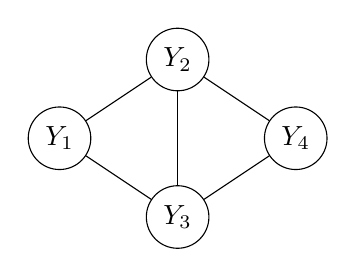
\begin{tikzpicture}
\node[draw,circle] (01) at (0,-1) {$Y_1$};
\node[draw,circle]  (10) at (1.5,0) {$Y_2$};
\node[draw,circle]   (12) at (1.5,-2) {$Y_3$};
\node[draw, circle]  (21) at (3,-1){$Y_4$};
\draw[-] (01) -- (10);
\draw[-] (01) -- (12);
\draw[-] (10) -- (12);
\draw[-] (21) -- (10);
\draw[-] (21) -- (12);
\end{tikzpicture}
\end{center}
\vspace{-0.4cm}
\caption{Example of a decomposable undirected graph with four vertices. \label{fig:UG}}
\end{figure}

\begin{example}
Consider the UG  with vertex set $\{Y_1,Y_2,Y_3,Y_4\}$ in Figure \ref{fig:UG}. The conditional independence statement associated to this graph is $
\ci{Y_4}{Y_1}{Y_2,Y_3,\bm{\theta}}$,
and therefore the associated density factorises as
\begin{equation*}
\label{eq:UGexamplefactorization}
f(\bm{y}\;|\;\bm{\theta})=\frac{f(y_1,y_2,y_3\;|\; \bm{\theta}_{[3]})f(y_2,y_3,y_4\;|\; \bm{\theta}_{[4]_1})}{f(y_2,y_3\;|\; \bm{\theta}_{[3]_1})},
\end{equation*}
or alternatively as 
\[
f(\bm{y}\;|\;\bm{\theta})=f(y_4\;|\; y_2,y_3, \bm{\theta}_4)f(y_1,y_2,y_3\;|\; \bm{\theta}_{[3]})=f(y_1\;|\; y_2,y_3, \bm{\theta}_1)f(y_2,y_3,y_4\;|\; \bm{\theta}_{[4]_1}).
\]
\end{example}

Just as in the directed case, conditions over the parameter vector can be imposed entailing distributed  inferences. For the purpose of this thesis we introduce only the strong hyper Markov condition of \citet{Dawid1993}.
\begin{definition}
\label{def:strongMarkov}
A density $\pi$ is strong hyper Markov for $\Gr$ if, for any decomposition $\{Y_i:i\in A\}$, $\{Y_i:i\in B\}$ of $\Gr$, $\bm{\theta}_A\independent \bm{\theta}_B$.
\end{definition} 
Since the cliques of a decomposable UG can be ordered to sequentially form a decomposition, we have the following result from \citet{Dawid1993}.
\begin{lemma}
\label{lemma:strongMarkov}
If a density $\pi$ for $\bm{\theta}$ is strong hyper Markov  then 
$
\pi(\bm{\theta})=\prod_{C\in\mathcal{C}}\pi(\bm{\theta}_{C}).$
\end{lemma}
We do not show in detail how to build a distribution exhibiting the strong hyper Markov condition. However we briefly note here that this can be straightforwardly done by considering the Markov combinations  of the marginal distributions over the cliques of the graph \citep{Massa2010}. 

The following proposition from \citet{Dawid1993} then shows how the strong hyper Markov condition is associated to fast distributed Bayesian inference.
\begin{proposition}
\label{prop:markovupdating}
Assume a vector $\bm{X}$ is sampled from the same population of $\bm{Y}$ and assume the density $\pi$ of $\bm{\theta}$ is strong hyper Markov. Then, the posterior distribution obtained by conditioning on the complete data $\bm{X}=\bm{x}$ is the unique strong hyper Markov distribution specified by the clique-marginal prior distributions given by $
\pi(\bm{\theta}_C\;|\; \bm{x})=f(\bm{x}_C\;|\;\bm{\theta}_C)\pi(\bm{\theta}_C).$
\end{proposition}
Therefore Bayesian updating can be performed locally within each clique whilst retaining the strong hyper Markov condition. Note that  the above result does not hold in general for non-decomposable undirected models. Whilst global independence is retained after observing certain incomplete datasets, strong hyper Markov laws are also broken by any incomplete observation. In Chapter \ref{chapter3} however we are able to show that for certain sets of incomplete observation the strong hyper Markov property can be retained if Bayesian updating is performed simultaneously for all the elements of this set.

We now consider the class of MN models whose associated distribution is Gaussian. A \emph{Gaussian MN} with decomposable UG $\Gr$, $V(\Gr)=\{Y_i:i\in[n]\}$, is defined as $\bm{Y}\;|\;\bm{\mu},\Sigma\sim \N(\bm{\mu},\Sigma)$, where $\bm{\mu}=(\mu_i)^\T_{i\in[n]}\in\mathbb{R}^n$ and $\Sigma$ is an $n\times n$ covariance matrix\footnote{A covariance matrix is a symmetric positive semidefinite matrix with entries in $\mathbb{R}_{>0}$ on the diagonal and in $\mathbb{R}$ otherwise.} such that if $(Y_i,Y_j)\not\in E(\Gr)\Longrightarrow \Sigma_{ij}^{-1}=0$, where $\Sigma_{ij}^{-1}$ is the entry of $\Sigma^{-1}$ in position $(i,j)$. So for example the covariance matrix associated to the Gaussian MN with graph in Figure \ref{fig:UG} is such that its inverse has zero entries in positions $(1,4)$ and $(4,1)$. Now for simplicity let $\bm{\mu}=\bm{0}$. Such a model class is usually referred to as a covariance selection model \citep{Wermuth1976}. Recall from Appendix \ref{sec:niw} that the Inverse Wishart distribution allows for conjugate learning with Normal models when defined as a prior of the covariance matrix. Let $\Sigma\sim \IW(A,d)$, where $A$ is a positive semidefinite $n\times n$ matrix and $d\in\mathbb{Z}_{\geq n}$. It is well known that for a subset $B\in[n]$, $\bm{Y}_{B}\sim \N(\bm{0},\Sigma_{B,B})$ and $\Sigma_{B,B}\sim \IW(A_{B,B},d)$, where, for a matrix $\Sigma$, $\Sigma_{B,B}$ is its submatrix with rows and columns $i\in B$ \citep[see e.g.][]{Dawid1993}. For every clique $C\in\mathcal{C}$ of $\Gr$, let $\bm{Y}_{C}\;|\;\Sigma_{C,C}\sim \N(\bm{0},\Sigma_{C,C})$ and assume the covariance  $\Sigma_{C,C}$ has an Inverse Wishart prior distribution $\IW(A^C,d)$. A unique strong hyper Markov distribution for the whole graph $\Gr$ having as marginals over the cliques these Inverse Wishart distributions exists if, calling $S_{ij}=C_i\cap C_j$, the matrices $A^{C_i}_{S_{ij},S_{ij}}$ and $A^{C_j}_{S_{ij},S_{ij}}$ are identical.\footnote{This result follows from Proposition 5.9 of \citet{Dawid1993} which we have not introduced here since it would require the introduction of additional concepts not relevant for the thesis. In a nutshell, this result is true because the Inverse Wishart is conjugate for the Normal covariance selection model and this distribution is a member of the exponential family.} We then say that $\Sigma$ follows an hyper Inverse Wishart distribution with parameters $A$ and $d$, $\Sigma\sim \HIW(A,d)$, where $A$ is such that $A_{C,C}=A^C$, for $C\in\mathcal{C}$.  

For the graph in Figure \ref{fig:UG}, let  $\Sigma_{[3],[3]}\sim \IW(A^{123},d)$ and $\Sigma_{[4]_1,[4]_1}\sim \IW(A^{234},d)$. Then an hyper Inverse Wishart distribution for this graph having this marginals exists if $A^{234}_{[3]_1,[3]_1}=A^{123}_{[3]_1,[3]_1}$.

Suppose now that a vector of observations $\bm{x}=(\bm{x}^\T_i)^\T_{i\in[m]}$ from the same family of $\bm{Y}$ has been collected, where $\bm{x}_i=(x_{ij})^\T_{j\in[n]}$. Assume an hyper Markov law is constructed from the clique marginals as exemplified above. Then from Appendix \ref{sec:niw} and Proposition \ref{prop:markovupdating} we know that for the covariance selection model the posterior density of $\Sigma\;|\;\bm{x}$ is strong hyper Markov, where each marginal over the submatrix associated with a clique $\Sigma_{C,C}$, $C\in\mathcal{C}$, follows an Inverse Wishart with parameters $A^C+mS_{C,C}$ and $d+m$, where $S$ is equal to $m^{-1}\sum_{i\in[m]}\bm{x}_i\bm{x}_i^\T$ (see Appendix \ref{sec:niw}). This can be easily noted within our example. The marginal posteriors over the cliques are $A^{123}\sim \IW(A^{123}+mS_{[3],[3]},d+m)$ and $A^{234}\sim \IW(A^{234}+mS_{[4]_1,[4]_1},d+m)$. It then holds that $A^{123}_{[3]_1,[3]_1}+mS_{[3]_1,[3]_1}=A^{234}_{[3]_1,[3]_1}+mS_{[3]_1,[3]_1}$, where
\begin{equation}
\label{stica}
mS_{[3]_1,[3]_1}=\left(
\begin{array}{cc}
\sum_{i\in[m]}x_{i2}^2&\sum_{i\in[m]}x_{i2}x_{i3}\\
\sum_{i\in[m]}x_{i2}x_{i3}&\sum_{i\in[m]}x_{i3}^2
\end{array}
\right)
\end{equation} 

\label{sec:UG}
\subsubsection{Probabilistic Chain Graphs.}
\label{sec:PCG}

Probabilistic Chain Graph (PCG) models are a hybrid representation of undirected and directed graphical models, allowing for the underlying graph $\Gr$ to be mixed and more specifically to be a Chain Graph (CG). We give here only a brief introduction to this class of models \citep[see e.g][for more details]{Cowell1999a, Frydenberg1990, Drton2009, Lauritzen1996a}. These are especially useful when there are both directional and non-directional relationships between the variables associated to the vertices of the underlying graph. As with the earlier models, we first introduce the relative Markov property, then derive the associated factorisation and in conclusion define the model. We let $Bd_i$ be the index set of the variables in the boundary of $Y_i$, $i\in[n]$.

\begin{definition}
A probability density $f$ over $\bm{Y}\;|\;\bm{\theta}$ is said to obey the chain Markov property relative to a CG $\Gr$ with vertex set $\{Y_i:i\in [n]\}$  and $m$ strong components if, for every vertex $Y_i$, $i\in[n]$,
$
Y_i\independent \bm{Y}_{A_i'\setminus Bd_i}\;|\; \bm{Y}_{Bd_i},\bm{\theta}$.
\end{definition}


\begin{proposition}
If a density $f$ obeys the chain Markov property relative to a CG $\Gr$ with vertex set $\{Y_i:i\in[n]\}$, then its density factorises as
\begin{equation*}
\label{eq:chainfactorization}
f(\bm{y}\;|\; \bm{\theta})= \prod_{i\in[m]} f\left(\bm{y}_{C_i}\;|\; \bm{y}_{\Pi_{C_i}}, \bm{\theta}_{C_i}\right),
\end{equation*}
where $C_1,\dots,C_m$ are the index sets of the variables in the strong components of $\Gr$ and $\Pi_{C_i}=\cup_{j\in C_i}\Pi_j$. 
\end{proposition}


We are now ready to formally define the model.
\begin{definition}
A PCG model consists of a CG $\Gr$ together with a density $f$ respecting the chain Markov property. 
\end{definition} 

\begin{figure}
\vspace{-0.2cm}
\begin{center}
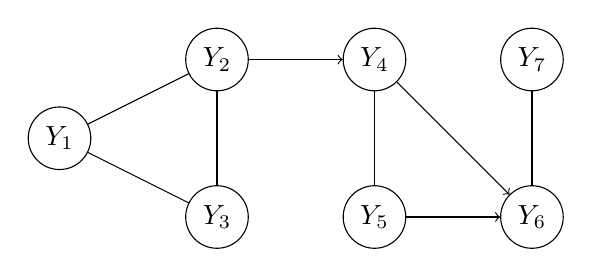
\begin{tikzpicture}
\node[draw,circle] (01) at (-1,-1) {$Y_1$};
\node[draw,circle] (10) at (1,0) {$Y_2$};
\node[draw,circle] (12) at (1,-2) {$Y_3$};
\node[draw,circle] (20) at (3,0) {$Y_4$};
\node[draw,circle] (22) at (3,-2) {$Y_5$};
\node[draw,circle] (32) at (5,-2) {$Y_6$};
\node[draw,circle] (30) at (5,0) {$Y_7$};
\draw[-] (01) -- (10);
\draw[-] (01) -- (12);
\draw[-] (10) -- (12);
\draw[->] (10) -- (20);
\draw[-] (20) -- (22);
\draw[->] (20) -- (32);
\draw[->]  (22) -- (32);
\draw[-]  (32) -- (30);
\end{tikzpicture}
\end{center}
\vspace{-0.2cm}
\caption{Example of a probabilistic chain graph model. \label{fig:CG}}
\end{figure}

\begin{figure}
\vspace{-0.2cm}
\begin{center}
\begin{tikzpicture}
\node[draw,ellipse, minimum height=1cm, minimum width=2cm,inner sep=0pt] (00) at (0,0) {$Y_1, Y_2,Y_3$};
\node[draw,ellipse, minimum height=1cm, minimum width=2cm,inner sep=0pt] (10) at (3,0) {$Y_4, Y_5$};
\node[draw,ellipse,minimum height=1cm, minimum width=2cm,inner sep=0pt](20) at (6,0) {$Y_6, Y_7$};
\draw[->] (00) -- (10);
\draw[->] (10) -- (20);
\end{tikzpicture}
\end{center}
\vspace{-0.4cm}
\caption{Representation of the chain graph in Figure \ref{fig:CG} as a directed acyclic graph. \label{fig:CGDAG}}
\end{figure}


\begin{example}
Consider the PCG in Figure \ref{fig:CG}. It can be deduced from this graph that the following conditional independence statements need to hold for a chain Markov distribution
\begin{equation*}
\begin{array}{lccl}
Y_4\independent Y_1,Y_3\;|\; Y_2,Y_5,\bm{\theta},&&& \ci{Y_5}{Y_1,Y_2,Y_3}{Y_4,\bm{\theta}}, \\
 Y_6\independent Y_1,Y_2,Y_3\;|\; Y_4,Y_5,Y_7,\bm{\theta},&&& \ci{Y_7}{Y_1,\dots,Y_5}{Y_6,\bm{\theta}},
\end{array}
\label{eq:examplechainindependence}
\end{equation*}
and the associated density can be factored as
\begin{equation*}
\label{eq:chainexamplefactorization}
f(\bm{y}\;|\; \bm{\theta})=f(y_6,y_7\;|\; y_4,y_5, \bm{\theta}_{67})f(y_4,y_5\;|\; y_3, \bm{\theta}_{45})f(y_1,y_2,y_3\;|\;\bm{\theta}_{123}).
\end{equation*}
\end{example}

Note that each PCG can be represented by a less expressive DAG whose vertex set corresponds to the strong components of the underlying CG. So for example the PCG in Figure \ref{fig:CG} can be transformed into the DAG of Figure \ref{fig:CGDAG}.
 
\subsubsection{Staged and Event Trees.}
\label{sec:tree}
All the classes of models defined so far are able  to depict standard conditional independence statements only. The class of \textit{event tree} models we discuss in this section is able to explicitly represent context specific independences. Event trees are such that their nodes are the situations in which a process might find itself and the edges emanating from a node are the possible unfoldings given the current situation. It has been extensively discussed in the literature that these models are extremely expressive in describing how processes might unfold. These are  especially useful in the cases where the variables are ordered in a way that follows the narrative of the events \citep{Shafer1996, Freeman2011, Smith2010}. 
 
Let $\mathcal{T}$ be a directed tree, $\Lambda(v,\mathcal{T})$ denote the set of paths from $v\in V(\mathcal{T})$ to a leaf node of $\mathcal{T}$ and $\mathcal{Y}=\Lambda(s_0,\mathcal{T})$, where $s_0$ is the root of the tree, be the set of root-to-leaf paths. Each path $y\in\mathcal{Y}$ is a so-called atomic event, i.e. a possible unfolding of events. Finally let $\mathcal{Y}_s$ denote the set of children of a situation $s\in S(\mathcal{T})$. 

\begin{definition}
An \textbf{event tree} is a directed tree $\mathcal{T}$ together with a random variable $Y_s$ for each situation $s\in S(\mathcal{T})$ with sample space $\mathcal{Y}_s$ defined conditional on having reached vertex $s$. The distribution of $Y_s$ is determined by the \emph{floret probability vector} $\bm{\theta}_s=(\theta_{ss'})^\T_{s'\in\mathcal{Y}_s}$, where  $\theta_{ss'}=\mathbb{P}(Y_s=s')$.
\end{definition}

\begin{figure}
\centerline{
\hspace*{-16mm} \xymatrixrowsep{0.5pc}{\xymatrixcolsep{2pc}
\xymatrix{
&&&&\bullet~v_{7}\\
&&&\bullet~v_{3}\ar@[red][r]_{\text{no}}\ar@[blue][ru]^{\text{yes}}&\bullet~v_{8}\\
&&\bullet~v_{1}\ar[r]_{\text{low}}\ar[ru]^{\text{high}}&\bullet~v_{4}\ar@[blue][r]|{\text{yes}}\ar@[red][rd]_{\text{no}}&\bullet~v_{9}\\
v_0\hspace*{-16mm}&\bullet\ar[ru]^{\text{yes}}\ar[rd]_{\text{no}}&&&\bullet~v_{10}\\
&&\bullet~v_{2}\ar[r]^{\text{high}}\ar[rd]_{\text{low}}&\bullet~v_{5}\\
&&&\bullet~v_{6}
}}}
\caption{Example of an event tree on three variables with the additional representation of its stages in different colors. \label{fig:ET}}
\end{figure}

The expressive power of event trees can be increased by identifying probabilities associated to different edges that are equal. Trees can then be embellished by a colouring of the edges, where two edges have same colour if their associated probabilities are equal.

\begin{definition}
A \textbf{staged tree} is an event tree where, for some $s
,s'\in S(\mathcal{T})$, the floret probability vectors are identified, $\bm{\theta}_s=\bm{\theta}_{s'}$, and equally coloured. Then $s$ and $s'$ are in the same \emph{stage}. We let $\mathbb{W}$ be the set of stages of $\mathcal{T}$.
\end{definition}
  

\begin{example}
\label{ex:staged}
Suppose a problem is modelled with three binary random variables: $Y_1$, release from a source term; $Y_2$, level of contamination in the surrounding area; $Y_3$, political disruption in the region due to the release. Suppose $\mathcal{Y}_1=\mathcal{Y}_3=\{\textnormal{yes},\textnormal{no}\}$ and $\mathcal{Y}_2=\{\textnormal{high},\textnormal{low}\}$. It is assumed that, if there has been a release, the level of contamination does not provide any information to predict the political disruption. This problem could then be modelled by a BN with vertex set $\{Y_1,Y_2,Y_3\}$ and edge set $\{(Y_1,Y_2), (Y_1,Y_3)\}$. 

However the BN representation forces us to retain information which is meaningless in this context, as for instance the atom (no,high,yes) which has probability zero. This is on the other hand explicitly modelled in the staged tree in Figure \ref{fig:ET}. In this tree the leftmost two edges are the possible outcomes of $Y_1$, the edges in the center are the outcomes of $Y_2$ given the different levels of $Y_1$, whilst the rightmost edges coincide with the outcomes of $Y_3$ given $Y_2$ and $Y_1$. In the lower part of the tree, associated to $Y_1=\textnormal{no}$, there are no outcomes for the political disruption variable, as these have probability zero. The set of situations of this tree includes vertices $\{v_0,\dots, v_6\}$ and leaves $\{v_{7},\dots, v_{10}\}$. Its stages are $w_0=\{v_0\}$, $w_1=\{v_1\}$, $w_2=\{v_2\}$, $w_3=\{v_3,v_4\}$. Furthermore $\mathbb{W}=\{w_0,\dots,w_3\}$. The tree representation of the associated BN model is in Figure \ref{fig:ETBN}. Such a tree is extremely regular in its colouring and each of its root to leaf paths have the same length: a property exhibited by the tree representation of any BN (see for more details Section \ref{sec:diff}).
\end{example}

\begin{figure}
\centerline{
\hspace*{-16mm} \xymatrixrowsep{0.5pc}{\xymatrixcolsep{2pc}
  \xymatrix{
&&&&\bullet~v_{7}\\
&&&\bullet~v_{3}\ar@[red][r]_{\text{no}}\ar@[blue][ru]^{\text{yes}}&\bullet~v_{8}\\
&&\bullet~v_{1}\ar[r]_{\text{low}}\ar[ru]^{\text{high}}&\bullet~v_{4}\ar@[blue][r]|{\text{yes}}\ar@[red][rd]_{\text{no}}&\bullet~v_{9}\\
v_0\hspace*{-16mm}&\bullet\ar[ru]^{\text{yes~}}\ar[rdd]_{\text{no}}&&&\bullet~v_{10}\\%
&&&&\bullet~v_{11}\\
&&\bullet~v_{2}\ar[rd]_{\text{low}}\ar[r]^{\text{high}}&\bullet~v_{5}\ar@[green][r]_{\text{no}}\ar@[brown][ru]^{\text{yes}}&\bullet~v_{12}\\
&&&\bullet~v_{6}\ar@[brown][r]|{\text{yes}}\ar@[green][rd]_{\text{no}}&\bullet~v_{13}\\
&&&&\bullet~v_{14}\\
}}}
\caption{Tree representation of the Bayesian network of Example \ref{ex:staged} .\label{fig:ETBN}}
\end{figure}

Although the colouring of the edges entails an improved representation of the overall structure of the problem at hand, conditional independences are still difficult to read from the graph. In addition as the number of variables increases, the size of the tree becomes quickly too large to be concisely reported. The class of models we introduce in the following section is able to compactly represent every conditional independence entertained.

\subsubsection{Chain Event Graphs.}
\label{sec:CEG}

Chain Event Graphs (CEGs) \citep{Smith2008} are models capable of representing context specific conditional independences in a single compact graphical representation. CEGs are constructed by starting with a staged tree, therefore requiring variables to be discrete, and then merging into a single vertex certain situations that are in the same stage. 

\begin{definition}
We say that two situations $s$ and $s'$ are in the same \emph{position} if the subtrees with roots $s$ and ${s'}$, respectively, have the same topology and the same edge colouring. We let $\mathbb{B}$ denote the set of positions of a staged tree.
\end{definition}

Note that two situations in the same position are by definition also in the same stage, whilst it does not necessary follows that two situations in the same stage are also in the same position. 

\begin{example}
 Considering the staged tree in Figure \ref{fig:ET}, we can see that for this example the set of stages coincides with the one of positions. 
\end{example} 
 
 \begin{definition}
 A \textbf{CEG} is the graph obtained by collapsing a staged tree into its positions. Its vertex set is equal to $\{\mathbb{B}\cup b_{\infty}\}$, where $b_{\infty}$ is the vertex collecting all the leaves of the tree. Its edge set is such that 
 \begin{itemize}
 \item there is an edge $(b_i,b_j)$, $b_i,b_j\in\mathbb{B}$, for every edge from a generic vertex $v\in b_i$ to any vertex $v'\in b_j$;
 \item there is an undirected edge between any two positions in the same stage;
 \end{itemize}
 \end{definition} 
 
\begin{example}
 The CEG representation of the staged tree of Figure \ref{fig:ET} is shown in Figure \ref{fig:CEG}, where we further annotated and coloured the edges as in \citet{Barclay2013a}. 
 \end{example}
 
\begin{figure}
\vspace{-.3cm}
\begin{center}
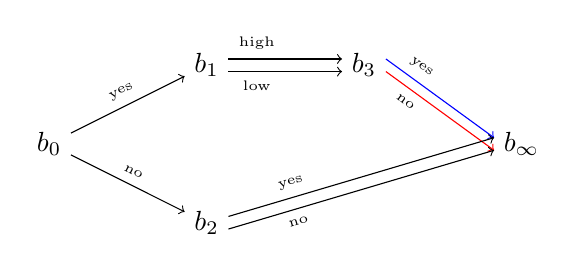
\begin{tikzpicture}
\node (00) at (0,0) {$b_0$};
\node (1-1) at (2,-1) {$b_2$};
\node (11) at  (2,1) {$b_1$};
\node (21) at (4,1) {$b_3$};
\node (30) at (6,0) {$b_{\infty}$};
\draw[->,sloped, anchor=center, above] (00) to  node {\tiny{yes}} (11);
\draw[->,sloped, anchor=center, above] (00) to  node {\tiny{no}} (1-1);
\draw[->,sloped, anchor=center, above,near start] ([yshift=0.08cm]11.east) to  node {\textcolor{black}{\tiny{high}}} ([yshift=0.08cm]21.west);
\draw[->,sloped, anchor=center, below,near start] ([yshift=-0.08cm]11.east) to  node {\textcolor{black}{\tiny{low}}} ([yshift=-0.08cm]21.west);
\draw[->,blue,sloped, anchor=center, above,near start] ([yshift=0.08cm]21.east) to  node {\textcolor{black}{\tiny{yes}}} ([yshift=0.08cm]30.west);
\draw[->,red,sloped, anchor=center, below,near start] ([yshift=-0.08cm]21.east) to  node {\textcolor{black}{\tiny{no}}} ([yshift=-0.08cm]30.west);
\draw[->,sloped, anchor=center, above,near start] ([yshift=0.08cm]1-1.east) to  node {\textcolor{black}{\tiny{yes}}} ([yshift=0.08cm]30.west);
\draw[->,sloped, anchor=center, below,near start] ([yshift=-0.08cm]1-1.east) to  node {\textcolor{black}{\tiny{no}}} ([yshift=-0.08cm]30.west);
\end{tikzpicture}
\end{center}
\vspace{-.5cm}
\caption{A chain event graph model representing the staged tree in Figure \ref{fig:ET}. \label{fig:CEG}}
\end{figure}

We chose the CEG as a representative model for context specific independences for two main reasons. First, compared to other models capable of  representing context specific conditional independences,  the CEG consists of a single graph. Furthermore   \citet{Smith2008} showed that every discrete BN can be represented as a CEG, whilst the converse does not hold. This is not case for example for probabilistic decision graphs \citep{Jaeger2004} and context specific BNs \citep{Boutilier1996}. \citet{Barclay2013a} nicely discussed how to convert a BN into a CEG model and how to measure the advantages of the latter representation. Second, a wide range of methods to perform various statistical analyses have been developed for this model class \citep[see e.g.][]{Barclay2013a,Barclay2014, Freeman2011, Thwaites2010, Thwaites2015}.

Importantly, under assumptions similar to local and global independence, but customised to staged trees and CEGs, Bayesian updating can be performed in a distributed way through the Multinomial-Dirichlet recursions illustrated in Appendix \ref{sec:multidir}. In Chapter \ref{chapter3} we generalise these independences for CEGs to take into account that probabilities over the graph are elicited by different groups of experts.  Suppose $w_i\in\mathbb{W}$ has $n_i$ emanating edges with associated probability vector $\bm{\theta}_i=(\theta_{ij})^\T_{j\in[n_i]}$, such that $\theta_{ij}\in(0,1)$ and $\sum_{j\in[n_i]}\theta_{ij}=1$, $j\in[n_i]$, $i\in[n]$. For a random sample $\bm{x}^\T=(\bm{x}_i^\T)_{i\in[n]}$, where $\bm{x}_i=(x_{ij})^\T_{j\in[n_i]}$ is the vector of the number of units that starts at stage $w_i$ and go through the emanating edges, it holds that
\begin{equation}
\label{eq:liktree}
f(\bm{x}\;|\;\bm{\theta})\propto\prod_{i\in[n]}\prod_{j\in[n_i]}\theta_{ij}^{x_{ij}},
\end{equation}
where we further assumed that $\bm{x}_i\independent \bm{x}_j\;|\;\bm{\theta}$, $i,j\in[n]$, and $\bm{\theta}^\T=(\bm{\theta}_i^\T)_{i\in[n]}$. Therefore the likelihood is multinomial. Now assuming $\bm{\theta}$ has mutually independent parameters, the independence  is retained a posteriori when the prior distribution is updated with the likelihood in equation (\ref{eq:liktree}). In particular this is conjugate if each stage probability vector $\bm{\theta}_i$ is given a Dirichlet prior distribution with parameter $\bm{a}_i=(a_{ij})^\T_{j\in[n_i]}\in\mathbb{R}^{n_i}_{>0}$. The posterior is then again Dirichlet with parameter $\bm{a}_i+\bm{x}_i$. \citet{Freeman2011} proved that assuming mutual independence of the parameters and some other fairly mild conditions, the prior distribution is necessarily Dirichlet.

\subsection{Dynamic Models}
\label{sec:dynmod}
In this section we deal with models for processes that are observed at several points in time, usually called \emph{time series}. The graphical models presented so far correspond to a fixed time, but now the random variables associated to the vertices of these will be allowed to vary in time, whilst, in most cases, the structure of the underlying graphical representation will remain constant through time. Such models allow for enough flexibility to represent situations where the relevant factors vary through time.

 Let $\{\bm{Y}_t\}_{t\in[T]}=\{Y_i(t):i\in[n]\}_{t\in[T]}$ be a $n$-dimensional time series with finite time horizon $T$, where $\{Y_i(t)\}_{t\in[T]}$, $i\in[n]$, is a univariate time series. We let $\mathcal{Y}_i$ and $\bm{\mathcal{Y}}=\bigtimes_{i\in[n]}\mathcal{Y}_i$ be the sample spaces of  $Y_i(t)$ and $\bm{Y}(t)$ respectively, for any $t\in[T]$. The density function of a generic $Y_i(t)$ is parametrised by  $\bm{\theta}_i(t)$ with sample space $\bm{\Theta}_i$. Let $\bm{Y}_A(t)^\T=(Y_i(t))_{i\in A}$, $\bm{Y}_A^t=(\bm{Y}_A(1)^\T,\dots,\bm{Y}_A(t)^\T )^\T$, $\bm{Y}_{[n]}(t)=\bm{Y}(t)$ and $\bm{\theta}_A^t=(\bm{\theta}_A(1)^\T,\dots, \bm{\theta}_A(t))^\T$, $A\subseteq[n]$. We denote with lower case letters instantiations of these random variables and vectors, and for any $t\in[T-1]$ the sample space of $(\bm{Y}(t),\bm{Y}(t+1))$ is $\bm{\mathcal{Y}}\bigtimes \bm{\mathcal{Y}}$. Finally, we denote with $I^t$ the information set at time $t$, which includes all the relevant information available to the DM. We assume in this section that $I^t=\{I^{t-1},\bm{Y}(t-1)\}$, $t\in[T]_1$.

\subsubsection{Dynamic Linear Models.}
\label{sec:DLM}
Based on a distributed version of the Kalman Filter \citep{Kalman1960}, the theory of Dynamic Linear Models (DLMs) was introduced in \citet{Harrison1976} and described in the seminal book of \citet{West1997}. This theory allows for a coherent updating of probabilities in dynamic frameworks, which can be then embedded within the graphical models we introduce in the following sections. The key property of such models is the underlying conditional independence structure which assumes that at each time point all the relevant evidence  is summarised in the distribution $\bm{\theta}(t)\;|\;\bm{\theta}(t{-1})$, where $\bm{\theta}(t)^\T=(\bm{\theta}_i(t)^\T)_{i\in[n]}$ has dimension $r$, and that consequently all the relevant information to predict $\bm{Y}(t)$ is synthesised in the distribution of $\bm{\theta}(t)$. This is depicted in Figure \ref{fig:CIDLM} implying, for each $t\in [T-1]_1$, $
\ci{\bm{Y}(t)}{I^{t-1}, \bm{\theta}^{t-1}}{\bm{\theta}(t)},$ and  $\ci{\bm{\theta}(t)}{I^{t-1}}{\bm{\theta}(t-1)}$.
 
\begin{figure}
\vspace{-.2cm}
\centerline{
\xymatrix{
&\bm{Y}(t-1)&\bm{Y}(t)&\bm{Y}(t+1)&\\
\ar[r]&\bm{\theta}(t-1)\ar[u]\ar[r]&\bm{\theta}(t)\ar[r]\ar[u]&\bm{\theta}(t+1)\ar[u]\ar[r]&
}}
\caption{Conditional independence structure underlying the dynamic linear model class. \label{fig:CIDLM}}
\end{figure} 

We now introduce the general form of the Normal DLM. 

\begin{definition}
\label{def:DLM}
The \emph{general Normal DLM} is defined by the following three equations.
\begin{align}
&\bm{Y}(t)=F(t)^{\T}\bm{\theta}(t)+\bm{v}(t),  &\bm{v}(t)&\sim \N\left(\bm{0},V(t)\right),\label{eq:obseq}\\
&\bm{\theta}(t)=G(t)\bm{\theta}(t-1)+\bm{w}(t),  &\bm{w}(t)&\sim \N\left(\bm{0},W(t)\right),\label{eq:evoeq}
\\
&\bm{\theta}(1)\;|\;I^0\sim \N\left(\bm{m}(0),C(0)\right),\nonumber \label{eq:ininfo}
\end{align}
where  $V(t)$, $W(t)$ and $C(0)$ are known covariance matrices of dimensions $n\times n$, $r\times r$ and $r\times r$, respectively, $F(t)$ and $G(t)$ are generic matrices of dimensions $n\times r$ and $r\times r$, respectively, $\bm{m}(0)\in\mathbb{R}^n$ and the errors $\bm{v}(1),\dots,\bm{v}(T), \bm{w}(1),\dots,\bm{w}(T)$ are mutually independent, where $\bm{v}(t)$ and $\bm{w}(t)$, $t\in[T]$, have dimension $n$ and $r$ respectively,  
\end{definition}

Equation (\ref{eq:obseq}) is the \textit{observation equation} specifying the distribution of $\bm{Y}(t)$ conditional on the \textit{system vector} $\bm{\theta}(t)$, having mean $F(t)^{\T}\bm{\theta}(t)$ and variance $V(t)$, also called \textit{observational variance matrix}. The matrix $F(t)$ is referred to as the \textit{regression matrix}, whilst $\bm{v}(t)$ is the \textit{observational error}. Equation (\ref{eq:evoeq}) is the \textit{system evolution equation}, which specifies how the values of the parameter vector evolve trough time. The matrices $G(t)$ and $W(t)$ are called respectively \textit{system transfer} and \textit{system variance} matrices. The vector $\bm{w}(t)$ is called \textit{system error}. 

Note that alternatively the general Normal DLM can be equivalently defined by substituting equations (\ref{eq:obseq})-(\ref{eq:evoeq}) with  the following two conditional distributional specifications:
\begin{equation*}
\label{eq:dlmdefinition}
\bm{Y}(t)\;|\;\bm{\theta}(t)\sim \N\left(F(t)^{\T}\bm{\theta}(t), V(t)\right),\;\;\;\;\;\;\;\; \bm{\theta}(t)\;|\; \bm{\theta}(t{-1}) \sim \N\left(G(t)\bm{\theta}(t-1),W(t)\right).
\end{equation*}

\begin{example}
Special cases of the general Normal DLM model are:
\begin{itemize}
\item a \textit{univariate DLM} is such that $\bm{Y}(t)$ has dimension $1$ (it is therefore a scalar);
\item a \textit{linear univariate DLM} is such that $F(t)=(1,X_{i}(t))_{i\in[r-1]}^\T$, where $X_{i}(t)$ is a regression variable, $i\in [r-1]$;
\item a univariate \textit{regression} DLM is such that the entries of $F(t)$ are generic functions of $X_{1}(t),\dots,X_{r-1}(t)$. 
\end{itemize}
\end{example}

Although we do not focus in this thesis on modelling issues, we note here that the theory of DLMs comprises a large variety of methodologies to model for example both seasonal and polynomial temporal trends. The concept of \textit{discount factors} is also widely used to elicit the values of the observational variance errors. Importantly, the conditional independence structure underlying DLMs provides a natural framework to \textit{intervene} on the system by for example changing the value of some of the model's parameters. This strategy is usually implemented when the model has a poor forecasting performance.

The assumption of Gaussianity in Definition \ref{def:DLM} is not strictly necessary but it entails some computational advantages. Under this assumption the updating equations of the parameters and the observables can be written in closed form and follow a Normal distribution, both in the univariate and the general case. The same property holds for the forecasting distributions, describing the behaviour of the system $k$-steps ahead in the future, for some $k\in\mathbb{Z}_{\geq 1}$. The associated recurrences when variances are known then reduce to the familiar Kalman Filter recurrences.

In practical applications the elicitation of the observational variance is critical and often prohibitive. However, there might be some information regarding its behaviour. Thus in practice $V(t)$ is often assumed unknown and a prior distribution is elicited. In the univariate case, an Inverse Gamma distribution can be given to this error, entailing a conjugate analysis as shown in Appendix \ref{sec:nig}. It is then possible to obtain closed recurrences for both the updating and the forecasting distributions which, unconditionally on V(t), follow a T-distribution (see again Appendix \ref{sec:nig}). Although we have shown in Appendix \ref{sec:niw} a conjugate analysis for the multivariate Normal model, this does not extend straightforwardly in a dynamic setting as in the univariate case to allow for sequential conjugate learning. We note here though that a variety of methods have been developed to approximate both numerically and analytically these recurrences \citep[see][]{West1997}. Most importantly in the following section we introduce a class of multivariate DLMs that entertains exact closed form updating and forecasting routines. 
  
\subsubsection{Multiregression Dynamic Models.}
\citet{Queen1993} introduced the class of \textit{Multiregression Dynamic Models (MDMs)}, multivariate DLMs exhibiting a conditional independence structure between the component time series which remains constant through time.  Although each variable is modelled through a simple univariate regression DLM, where the regressors are specified by the conditional independence structure, the model class of MDMs is in general non Gaussian. The qualitative structure underlying an MDM can be represented through a DAG whose vertices are the component time series. Importantly, the well known BN model we reviewed in Section \ref{sec:BN} is a special case of the MDM.

\begin{definition}
\label{def:MDM}
An \emph{MDM} for the time series $\{\bm{Y}(t)\}_{t\in[T]}$ is defined by a DAG $\Gr$ with vertex set $\{Y^T_i:i\in[n]\}$ together with the following $n$ observation equations, system equation and initial information:
\begin{equation*}
\begin{array}{llc}
Y_i(t)=\bm{F}_i(t)^\T\bm{\theta}_i(t)+v_i(t),&v_i(t)\sim (0,V_i(t)),&i\in[n];\\
\bm{\theta}(t)=G(t)\bm{\theta}(t-1)+\bm{w}(t)&\bm{w}(t)\sim(0,W(t));&\\
\bm{\theta}(0)\;|\; I^0\sim (\bm{m}(0),C(0)).
\end{array}
\end{equation*}

The system vector is $\bm{\theta}_i(t)\in\mathbb{R}^{r_i}$  and $\bm{F}_i(t)$, of dimension $r_i$, is an arbitrary function of $\bm{y}^t_{\Pi_i}$ and $\bm{y}^{t-1}_i$, but  not $\bm{y}^t_{De_i}$ and $y_i(t)$.  The scalar observation variances  $V_i(t)\in\mathbb{R}_{>0}$, $i\in[n]$, can be either known or unknown. The $r\times r$ matrices, $r=\sum_{i=1}^n r_i$, $G(t)=\textnormal{blockdiag}(G_1(t),\dots,G_n(t))$,  $W(t)=\textnormal{blockdiag}(W_1(t),\dots,W_n(t))$ and   $C_0=\textnormal{blockdiag}(C_1(0),\dots,C_n(0))$, are assumed known and such that $W_i(t)$ and $C_i(t)$ are covariance matrices, whilst $G_i(t)$ is a generic matrix, all of dimension $s_i\times s_i$, $i\in [n]$.\footnote{$\blockdiag$ denotes a block-diagonal matrix.} The errors $v_1(t),\dots,v_n(t),\bm{w}_1(t),\dots,\bm{w}_n(t)$, where $\bm{w}_i(t)\sim(\bm{0},W_i(t))$, are mutually independent.
\end{definition} 

\begin{example}
Consider a time series $\{\bm{Y}(t)\}_{t\in[T]}=\{Y_1(t),Y_2(t),Y_3(t),Y_4(t)\}_{t\in[T]}$. An MDM having the conditional independence structure depicted by the DAG in Figure \ref{fig:MDM} would have observation equations in which $\bm{F}_1(t)$ is a function of $\bm{y}^{t-1}_1$ and, for $i\in[4]_1$, $\bm{F}_i(t)$ is a function of $y^{t}_{i-1}$ and $y^{t-1}_i$. 
\end{example}

\begin{figure}
\vspace{-.2cm}
\centerline{
\entrymodifiers={++[o][F-]}
\xymatrix{
\bm{Y}^T_1\ar[r]&\bm{Y}^T_2\ar[r]&\bm{Y}^T_3\ar[r]&\bm{Y}^T_4
}
}
\caption{A directed acyclic graph associated to the conditional independence structure of a multiregression dynamic model. \label{fig:MDM}}
\end{figure}

We now report from \citet{Queen1993} two key results associated to MDMs. For ease of notation we assume the observational variances to be known, but these results straightforwardly generalise to the case of unknown observational variances. 

\begin{proposition}
\label{prop:MDM}
For an MDM over a time series $\{Y_i(t):i\in[n]\}_{t\in[T]}$, we have that 
$\independent_{i\in[n]}\bm{\theta}_i(t)\;|\; \bm{y}^{t-1}$  and $
\ci{\bm{\theta}_i}{\bm{y}^t_{[n]\setminus Fa_i}}{\bm{y}_{Fa_i}^t}$.
\end{proposition}
The first conditional independence in Proposition \ref{prop:MDM} indicates that the parameters associated to different component time series remain independent of each other through time. The second one guarantees that a parameter $\bm{\theta}_i(t)$, given the past observations of the variables with indices in the family set, is independent of the rest of the observed data. We show in Chapter \ref{chapter3} that these independences guarantee the MDM is an ideal model for the aggregation of expert judgements in the class of problems we address in this thesis.

Because of these results, we note that the overall updating of the multivariate time series can be performed locally for each of the component time series independently. Each of these follows, conditionally on the series with indices in the parent set, a simple univariate regression DLM. Therefore all the technology briefly reviewed in Section \ref{sec:DLM}, as for example intervention and seasonal trends, can be directly transferred into MDMs. 

Note that there is no assumption of Gaussianity in the definition of the MDM. However a \textit{Normal MDM} can be defined such that the errors $v_t(i)$ and $\bm{w}_t$ follow a Gaussian distribution. In such cases the overall distribution is non Gaussian, but the forecasting and updating distributions can still be computed analytically and in closed form using the DLM machinery. Therefore MDMs, although being multivariate DLMs, do not need any approximated method. The following proposition formalises this fundamental observation.

\begin{proposition}
\label{prop:MDM2}
For an MDM over a time series $\{Y_i(t):i\in[n]\}_{t\in[T]}$, it holds that 
\begin{equation}
\label{eq:mdmeq1}
f(\bm{y}(t),\bm{\theta}(t)\;|\; I^{t-1})=\prod_{i\in[n]}f(y_i(t)\;|\;\bm{y}_{\Pi_i}(t),\bm{\theta}_i(t), I^{t{-1}})\pi(\bm{\theta}_i(t)\;|\;I^{t-1}).
\end{equation}
and 
\begin{equation}
 \label{eq:mdmmarg}
 f\left(\bm{y}(t)\;|\;\bm{y}^{t-1}\right)=\prod_{i\in[n]} g_{t,i}\left(\bm{y}^t_{Fa_i},\bm{\theta}_i(t)\right),
 \end{equation}
where
\begin{equation}
g_{t,i}=\int_{\bm{\Theta}_i}f\left(y_i(t)\;|\;\bm{y}^{t}_{\Pi_i},\bm{y}^{t-1}_i,\bm{\theta}_i(t)\right)\pi\left(\bm{\theta}_i(t)\;|\;\bm{y}^{t-1}_{Fa_i}\right)\textnormal{d} \bm{\theta}_t(i).
\label{eq:mdmeq2}
\end{equation}
\end{proposition}
 Proposition \ref{prop:MDM} is a generalisation of the distributed learning property in BNs under the assumption of global independence we formalised in Proposition \ref{prop:ancupd}.
\begin{example}
For the MDM in Figure \ref{fig:MDM}, equation (\ref{eq:mdmeq1}) can be written as, letting $I=I^{t-1}$ for ease of notation,
\begin{equation*}
\label{eq:factorizationMDMexample}
f(\bm{y}(t),\bm{\theta}(t)\;|\; I)=f(y_1(t)\;|\;\bm{\theta}_1(t),I)\prod_{i\in[4]_1}f(y_i(t)\;|\;\bm{\theta}_i(t),y_{i-1}(t),I)\prod_{j\in[4]}\pi(\bm{\theta}_j(t)\;|\;I).
\end{equation*}
The terms in equation (\ref{eq:mdmeq2}) appearing in the forecasting distribution of equation (\ref{eq:mdmmarg}) can be written for this example as
\begin{equation*}
g_{t,i}= 
\left\{
\begin{array}{ll}
\!\!\!\!\int_{\bm{\Theta}_i}f\left(y_i(t)\;|\; \bm{y}^{t-1}_i,\bm{\theta}_i(t)\right)\pi\left(\bm{\theta}_i(t)\;|\; \bm{y}^{t-1}_i\right)\dr \bm{\theta}_i(t), & i=1,\\
\!\!\!\!\int_{\bm{\Theta}_i}f\left(y_i(t)\;|\; \bm{y}^{t-1}_i,\bm{y}^t_{i-1},\bm{\theta}_i(t)\right)\pi\left(\bm{\theta}_i(t)\;|\; \bm{y}^{t-1}_i,\bm{y}^{t-1}_{i-1}\right)\dr \bm{\theta}_i(t), & i\in[4]_1.
\end{array}
\right.
\label{eq:exampleMDMpredictive}
\end{equation*}
\end{example}

We now introduce a special case of the MDM class, the \textit{linear MDM} \citep{Queen1993}, which is very simple to work with. 

\begin{definition}
A \emph{Linear Multiregression Dynamic Model (LMDM)} is an MDM where the errors are assumed to be Gaussian and each component time series is modelled as a univariate linear DLM.
\end{definition}
In an LMDM, at each time point, each $Y_i(t)$ is modelled as a linear regression with the contemporaneous parent variables as regressors. Therefore the LMDM is a dynamic extension of the Gaussian BN model introduced in Proposition \ref{proposition:ciao2}. 

\begin{example}
The observation equations of an LMDM respecting the DAG in Figure \ref{fig:MDM} (and using an obvious generalisation of the notation in equation (\ref{eq:GausBN})) are as follows
\begin{align}
&Y_1(t)=\theta_{01}(t)+v_1(t), &Y_2(t)=\theta_{02}(t)+\theta_{12}(t)Y_1(t)+v_2(t),\nonumber\\
&Y_3(t)=\theta_{03}(t)+\theta_{23}(t)Y_2(t)+v_3(t),&Y_4(t)=\theta_{04}(t)+\theta_{34}(t)Y_3(t)+v_4(t).\nonumber
\end{align}
\end{example}
\citet{Queen1993} and \citet{Queen2008} described methods to analytically compute the first two moments of $\bm{Y}(t)$ under the assumption of an LMDM. These simply consist of a sequential use of the tower properties of the first two moments. Many of the results we present in the following chapters use similar techniques.

Because of its independence properties and its flexibility, the MDM has now been successfully applied in practice in many diverse domains: traffic flows \citep{Anacleto2013}, biology \citep{Oates2013}, brain connectivity \citep{Costa2015}, brand sales \citep{Queen1994} and finance \citep{Zhao2015}. Furthermore, a wide tool-kit of more advanced modelling techniques has now been implemented within MDMs to allow for causal reasoning \citep{Queen2009}, model choice and averaging \citep{Costa2015,Zhao2015} and heteroscedasticity \citep{Anacleto2013}. 

\subsubsection{Dynamic Chain Graphs.}
\label{sec:DCG}
Although the MDM allows for great flexibility in modelling multivariate dynamic domains, its underlying DAG structure implies the presence of directional associations only and does not allow for any symmetric relationship. To address this issues, \citet{Queen1992} and \citet{Anacleto2013c} developed the \textit{Dynamic Chain Graph (DCG)} model, a multivariate DLM whose underlying conditional independence structure can be represented by a CG. 

For the purpose of this section only, let $\bm{Y}(t)$ be partitioned into $N$ vector time series of dimensions $n_1,\dots,n_N$, $\sum_{i\in[N]}n_i=n$, so that $\bm{Y}(t)^\T=(\bm{Y}_i(t)^\T)_{i\in[N]}$ where $\bm{Y}_i(t)^\T=(Y_{ij}(t))_{j\in[n_i]}$. Let $\bm{Y}_{ij}^t=(Y_{ij}(1),\dots,Y_{ij}(t))^\T$. Suppose the independence structure is such that any two $\bm{Y}_{ij}^T$ and $\bm{Y}_{ik}^T$ are connected by an undirected edge in the underlying CG, $j,k\in [n_i]$, $i\in [N]$. 

\begin{definition}
A \emph{DCG} consists of a CG $\Gr$, $V(\Gr)=\{Y_{ij}^T:i\in[N],j\in[n_i]\}$, together with the following $N$ observations equations, system equation and initial information:
\begin{equation*}
\begin{array}{lll}
\bm{Y}_i(t)=\bm{F}_i(t)^\T\bm{\theta}_i(t)+v_i(t),&\bm{v}_i(t)\sim(\bm{0},V_i(t)), &i\in [N],\\
\bm{\theta}(t)=G(t)\bm{\theta}(t{-1})+\bm{w}(t), & \bm{w}(t)\sim(\bm{0},W(t)),&\\
\bm{\theta}(1)\;|\;I(0)\sim (\bm{m}(0),C(0)).
\end{array}
\end{equation*}
The vector $\bm{F}_i(t)^\T=\left(\bm{F}_{ij}(t)^\T\right)_{j\in[n_i]}$ includes the subvectors $\bm{F}_{ij}(t)\in\mathbb{R}^{r_{ij}}$ known functions of $\bm{y}^{t-1}_i$ and $\bm{y}^t_{\Pi_{ij}}$, where $\Pi_{ij}$ is the set of the indices of the parents of $\bm{Y}_{ij}^T$ in $\Gr$, $j\in[n_i]$. The system vector $\bm{\theta}(t)^\T=(\bm{\theta}_i(t)^\T)_{i\in[N]}\in\mathbb{R}^r$, where $\bm{\theta}_i(t)\in\mathbb{R}^{r_i}$ is the system vector of $\bm{Y}_i(t)$, with $r_i=\sum_{j\in[n_i]}r_{ij}$ and $r=\sum_{i\in[N]}r_i$. The $n_i\times n_i$ covariance matrix $V_i(t)$ is the observational variance for $\bm{Y}_i(t)$. The $r\times r$ matrices $G(t)=\blockdiag(G_1(t),\dots,G_N(t))$, $W(t)=\blockdiag(W_1(t),\dots,W_N(t))$ and $C(0)=\blockdiag(C_1(0),\dots,C_N(0))$ are assumed known and such that  $W_i(t)$ and $C_i(0)$ are $r_i\times r_i$ covariance matrices and $G_i(t)$ is a generic matrix. The errors $\bm{v}_1(t),\dots, \bm{v}_N(t),\bm{w}_1(t),\dots,\bm{w}_N(t)$, $\bm{w}_i(t)\sim \N(\bm{0},W_i(t))$, are assumed mutually independent. 
\end{definition}

\begin{figure}
\vspace{-0.2cm}
\begin{center}
\scalebox{0.95}{
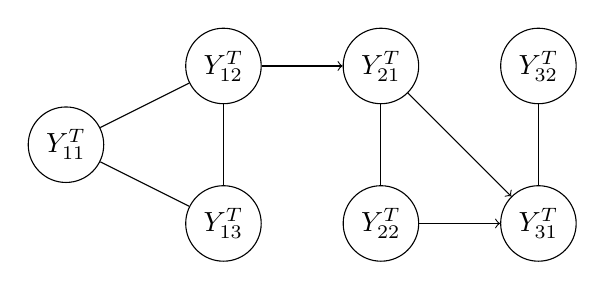
\begin{tikzpicture}[node distance= 2.5cm]
\node[draw,circle] (01) at (-1,-1) {$\bm{Y}_{11}^T$};
\node[draw,circle] (10) at (1,0) {$\bm{Y}_{12}^T$};
\node[draw,circle] (12) at (1,-2) {$\bm{Y}_{13}^T$};
\node[draw,circle] (20) at (3,0) {$\bm{Y}_{21}^T$};
\node[draw,circle] (22) at (3,-2) {$\bm{Y}_{22}^T$};
\node[draw,circle] (32) at (5,-2) {$\bm{Y}_{31}^T$};
\node[draw,circle] (30) at (5,0) {$\bm{Y}_{32}^T$};
\draw[-] (01) -- (10);
\draw[-] (01) -- (12);
\draw[-] (10) -- (12);
\draw[->] (10) -- (20);
\draw[-] (20) -- (22);
\draw[->] (20) -- (32);
\draw[->]  (22) -- (32);
\draw[-]  (32) -- (30);
\end{tikzpicture}}
\end{center}
\vspace{-.4cm}
\caption{Dynamic variant of the chain graph model in Figure \ref{fig:CG}. \label{fig:DCG}}
\end{figure}

\begin{example}
Consider the DCG defined by the CG of Figure \ref{fig:DCG}. Since the topology of this CG is the same as the one in Figure \ref{fig:CG}, this DCG has three strong components, corresponding, for each time slice $t\in[T]$, to $\bm{Y}_1(t)=(Y_{11}(t),Y_{12}(t),Y_{13}(t))^\T$, $\bm{Y}_{2}(t)=(Y_{21}(t),Y_{22}(t))^\T$ and $\bm{Y}_{3}(t)=(Y_{31}(t),Y_{32}(t))^\T$. Note that in this case we have $\bm{Y}(t)^\T=(\bm{Y}_1(t)^\T,\bm{Y}_2(t)^\T,\bm{Y}_3(t)^\T)$, as confirmed by Figure \ref{fig:CGDAG}. The observation equations are specified by the following vectors: $\bm{F}_1(t)^\T=(\bm{F}_{11}(t)^\T,\bm{F}_{12}(t)^\T,\bm{F}_{13}(t)^\T)$, functions of $\bm{y}^{t-1}_1$; $\bm{F}_2(t)^\T=(\bm{F}_{21}(t)^\T,\bm{F}_{22}(t)^\T)$, functions of $\bm{y}^{t-1}_2$, where $\bm{F}_{21}(t)$ is also a function of $\bm{y}^t_{13}$; $\bm{F}_3(t)^\T=(\bm{F}_{31}(t)^\T,\bm{F}_{32}(t)^\T)$, function of $\bm{y}^{t-1}_3$, where $\bm{F}_{31}(t)$ is also a function of $\bm{y}^t_2$. 
\end{example}

It can be shown that the results in Propositions \ref{prop:MDM} and \ref{prop:MDM2} for MDMs hold for DCGs if applied to the chain component observation series $\bm{Y}_i(t)$ and their associated system vectors $\bm{\theta}_i(t)$,  $i\in [N]$. Therefore in DCGs the sequential updating and forecasting of the  relevant probabilities can be distributed across the chain components of the underlying CG. 

\subsubsection{Dynamic Bayesian Networks.}
The two described multivariate models are not as commonly used in practice as the \textit{Dynamic Bayesian Network (DBN)} model class \citep{Murphy2002}. DBNs extend the BN framework to dynamic and stochastic domains. We discuss these models in this thesis to provide an example of a model class whose conditional independence structure is not retained as time progresses and therefore do not enjoy closed form updating routines.

 For the purpose of this thesis, and as often in practice, we consider only stationary, feed-forward DBNs respecting the first order Markov assumption \citep[see e.g.][]{Oates2013}. These DBNs can be simply described by an initial distribution over the first time point and a BN having as vertex set two generic time slices. Such latter BN is usually called 2-Time slice Bayesian Network (2-TBN).

\begin{definition}
\label{def:2-TBN}
A \emph{2-TBN} for $\{\bm{Y}(t)\}_{t\in[T]}$ is a BN with DAG $\Gr$ such that, fixed a  $t\in [T-1]$, $V(\Gr)=\{Y_i(t),Y_{i}(t+1):i\in[n]\}$, any vertex $Y_i(t)$ has no parents and there are no edges $(Y_{i}(r),Y_{j}(r))$, $i,j\in[n]$, $r=t,t+1$.   
\end{definition} 
    
\begin{figure}
\vspace{-.3cm}
\centerline{
\entrymodifiers={++[o][F-]}
\xymatrix{
Y_1(t)\ar[d]&Y_2(t)\ar[d]\ar[dl]&Y_3(t)\ar[d]\ar[dl]&Y_4(t)\ar[d]\ar[dl]\\
Y_{1}(t{+1})&Y_{2}(t{+1})&Y_{3}(t{+1})&Y_{4}(t{+1})
}
}
\caption{Example of a 2-time-slice Bayesian network for a multivariate time series comprising four univariate series. \label{fig:2-TBN}}
\end{figure}

\begin{definition}
A \emph{DBN} for the time series $\{\bm{Y}(t)\}_{t\in[T]}$ is a pair $(\Gr,\Gr')$, such that $\Gr$ is a BN with vertex set $V(\Gr)=\{Y_i(1):i\in[n]\}$, and $\Gr'$ is a 2-TBN such that its  vertex set $V(\Gr')$ is equal to $\{Y_i(t),Y_{i}(t+1):i\in[n]\}$.
\end{definition}

It is therefore straightforward to notice that a recursive formula for the density function of a DBN similar to the one for BNs in Lemma \ref{lemma:rec} exists. This is because a DBN can be thought of as the concatenation of BNs.

\begin{example}
\label{ex:DBN}
The BN in Figure \ref{fig:2-TBN} is a valid 2-TBN because its topology respects the conditions of Definition \ref{def:2-TBN}. Suppose a DBN has such 2-TBN and the BN associated to the initial distribution over $\bm{Y}(1)$ has empty edge set, i.e. represents the independence model in Definition \ref{def:indmodel}. Then its probability density function factorises as (suppressing the dependence on the parameter vector for ease of notation)
\begin{equation*}
\label{eq:exampleDBNfactorization}
f\left(\bm{y}^T\right)=\prod_{i\in[4]}f(y_i(1))\prod_{t\in[T]_1}f(y_4(t)\;|\;y_{4}(t{-1}))\prod_{j\in[3]}f(y_j(t)\;|\;y_{j}(t{-1}),y_{j+1}(t{-1}))
\end{equation*}
\end{example}

Although DBNs entail an effective recursive factorisation of the associated density function, thus requiring a low number of probabilities to be elicited in order to fully specify the model, inference in such models cannot be performed as easily as in both BNs and MDMs. This is because the initial conditional independence structure is broken through time. As shown in Figure \ref{fig:unrolled} \citep[from ][]{Boyen1998}, the so-called unrolled version of the DBN of Example \ref{ex:DBN}, after a small number of time steps all the variables in a same time slice become correlated with each other. Independence can only be retained if each component time series is independent of the others, i.e. if the 2-TBN has edges of the type $(Y_i(t),Y_i(t+1))$ and an initial distribution described by an independence model. Therefore the efficient and distributed recursions for both inference and forecasting associated to MDMs and DCGs do not transfer to generic DBNs. This is the reason why DBNs are not an effective model class for exact aggregation methods in the problems we address in Chapter \ref{chapter3}. However, we note here that a variety of methodologies based on stochastic approximated methods have been developed for tractable inferences in such models \citep{Boyen1998, Koller2001}. 

\begin{figure}
\vspace{-.3cm}
\centerline{
\scalebox{0.75}{
\entrymodifiers={++[o][F-]}
\xymatrix{
Y_1(1)\ar[r]&Y_1(2)\ar[r]&Y_1(3)\ar[r]&Y_1(4)\\
Y_2(1)\ar[r]\ar[ur]&Y_2(2)\ar[r]\ar[ur]&Y_2(3)\ar[r]\ar[ur]&Y_2(4)\\
Y_3(1)\ar[r]\ar[ur]&Y_3(2)\ar[r]\ar[ur]&Y_3(3)\ar[r]\ar[ur]&Y_3(4)\\
Y_4(1)\ar[r]\ar[ur]&Y_4(2)\ar[r]\ar[ur]&Y_4(3)\ar[r]\ar[ur]&Y_4(4)}}}
\caption{Unrolled version of the dynamic Bayesian network of Example \ref{ex:DBN} with 2-time-slice Bayesian network of Figure \ref{fig:2-TBN}.\label{fig:unrolled}}
\end{figure}

\subsection{Causality}
\label{sec:causality}
Statistical reasoning has historically largely avoided  investigating causal inferences. Classical methods, as for example regression analysis, are in general only able to predict new values of a variable given the values of a set of covariates, and how these relate to the response variable. Until recently, there has not been a formal study of causal relationships between sets of random variables to assess, for example, whether a variable can be considered as a \textit{cause} for another one or not. However, artificial intelligence researchers such as \citet{Pearl2000} and \citet{Spirtes1993}, provided a systematic study of the causal mechanisms underlying a given hypothesised BN model when certain variables are \textit{manipulated} and fixed to take a certain value in their sample space. This theory supposes the existence of an underlying idle system, i.e. one where its variables are observed and not manipulated to a certain value. 
 
We introduce here the concept of causality since, for the purpose of decision support, it is often helpful to match data coming from experiments in a laboratory, where variables are held fixed to a particular value, to observational one, to provide a revised and more focused specification of the relevant probabilities. 
 
\citet{Shafer1996} discusses causal reasoning for models depicted by trees. As also suggested by \citet{Smith2010}, trees are particularly suitable to represent causal relationships, since these can uniquely describe the actual narrative underlying the unfolding of events. We also note here that causal reasoning is more tenable for Bayesian decision analysis than in pure inferential reasoning since DMs need to think hard on how the problem at hand unfolds when eliciting both their probabilistic and preferential beliefs. Therefore, a DM's model can often be used to answer various causal questions \citep{Smith2010}.

We now formally define the concept of intervention as introduced in \citet{Pearl2000}.

 \begin{definition}
 A \emph{Perlean intervention} on $\bm{Y}_A$, $A\subset[n]$, consists of fixing these variables to a (known) value $\bm{y}_A$. The resulting density is written $f\left(\bm{y}\;|\;\do(\bm{Y}_A=\bm{y}_A)\right)$.
 \end{definition} 

As noted in Section \ref{sec:BN}, there are several BNs entertaining the same density factorisation and therefore leading to the same kind of inferences. Causal reasoning cannot thus be straightforwardly followed in generic BNs. We define here a particular class of BNs that are causal in the Perlean sense.

\begin{definition}
\label{def:cbn}
A BN $\Gr$ is a \emph{Causal Bayesian Network (CBN} if, for any Perlean intervention on $\bm{Y}_A$, $A\subset[n]$, it holds that 
\begin{equation*}
f\left(\bm{y}\;|\;\bm{\theta},\do(\bm{Y}_A=\bm{y}_A)\right)=\prod_{i\in[n]\setminus A}f\left(y_i\;|\;\bm{\theta}_i,\bm{y}_{\Pi_i}\right).
\end{equation*} 
\end{definition} 

\begin{example}
Consider the CBN with DAG in Figure \ref{fig:BNexample}. Suppose we intervene on this DAG and set $Y_2=y_2$. The resulting factorisation is equal to
\begin{equation*}
f\left(y_1,y_2,y_3,y_4\;|\;\bm{\theta},do(Y_2=y_2)\right)=f(y_1\;|\;\bm{\theta}_1)f(y_3\;|\;y_1,y_2,\bm{\theta}_3)f(y_4\;|\;y_1,\bm{\theta}_4).
\end{equation*}
Such intervention can be depicted graphically by deleting every edge into $Y_2$, in this case simply $(Y_1,Y_2)$, and changing the label of the vertex associated to the intervened variable to $Y_2=y_2$. Such DAG is reported in Figure \ref{figure:causalBN}.
\end{example}

\begin{figure}
\vspace{-.2cm}
\entrymodifiers={++[o][F-]}
\centerline{
\xymatrix{
\mbox{\large{$Y_4$}}&\mbox{\large{$Y_2=y_2$}}\ar[d]\\
\mbox{\large{$Y_1$}}\ar[u]\ar[r]&\mbox{\large{$Y_3$}}
}
}
\vspace{-.2cm}
\caption{
Causal version of the Bayesian Network in Figure \ref{fig:BNexample} under the intervention $Y_2=y_2$. \label{figure:causalBN}}
\end{figure}

\begin{definition}
For an intervention $\do(\bm{Y}_A=\bm{y}_A)$ over the variables of a CBN $\Gr$, $V(\Gr)=\{Y_i:i\in[n]\}$, we call \emph{manipulated DAG} $\Gr'$ the network with edge set $\E(\Gr')=\E(\Gr)\setminus\{(Y_i,Y_j)\in E(\Gr): j\in A\}$ and $V(\Gr')=\{Y_i: i\in \{[n]\setminus A\}\}\cup \{Y_i=y_i: i\in A\}$.
\end{definition}

If a BN is believed to be causal, then experimental evidence can be used to update the parameter densities as formalised below.

\begin{proposition}
 Suppose global independence holds and assume the experimental sample $\bm{x}$ from the same population as $\bm{Y}$ is ancestral with respect to the manipulated DAG for the intervention $do(\bm{Y}_A=\bm{y}_A)$. Let $I$ be the set of indices of both the vertices whose children are not sampled and the leaves of the DAG. Then, for a CBN the posterior factorises as
 \begin{equation*}
 \pi(\bm{\theta}\;|\;\bm{x})=\prod_{i\in I}\prod_{\substack{j\in A_i\\j\not\in A}}\pi(\bm{\theta}_j\;|\;\bm{x})\prod_{k\not\in \{A_i\cup A\}}\pi(\bm{\theta}_k).
 \end{equation*}
\end{proposition}

The concept of causality for BNs has been extended in \citet{Daneshkhah2004} to take into account manipulations of the parameter vector, usually called \textit{randomised interventitions} \citep[see e.g.][]{Lauritzen2001, Daneshkhah2004}.  These consist of fixing a random parameter of the density of a random variable to take a particular known value.   \citet{Daneshkhah2004} defined the concept of an hypercausal BN, which is one where certain randomised interventions respect the topology of the DAG. Most importantly they showed that local and global independence holds iff the BN is hypercausal and therefore also in the case the model is a CBN. Thus the validity of the causal assumption can be checked through reasoning about the faithfulness of global and local independence and vice versa. In Chapter \ref{chapter3} below we define a new class of randomised interventions related to committing to a countermeasure policy. We are able to show that Perlean interventions in CBNs can be seen as a special case of our methodology.  
 
We have focused here on causality over graphical directed structures, since these naturally provide a framework for causal reasoning. In these models variables are ordered and there are no symmetric relationships. This is the reason why causal arguments in MN models are much more difficult to develop \citep[see e.g.][]{Lauritzen2002}. Although much of the literature on statistical causality centred on the BN model class, the causal semantic has been extended to a variety of frameworks, e.g. CEGs \citep{Thwaites2010,Thwaites2013}, CGs \citep{Lauritzen2002}, DBNs \citep{Eichler2007}, IDs \citep{Dawid2002a}, MDMs \citep{Queen2009} and  others \citep{Aalen2012, Dawid2010, Smith2007}.  We point out that \citet{Dawid2010} developed causal arguments in the framework of \textit{dynamic treatment strategies} \citep{Murphy2003}. These are dynamic models in medical contexts where the objective is to identify the causal effect of a particular treatment. The computation of these effects is based on backward inductive arguments, which mirror the recursions we develop in Chapter \ref{chapter4} for IDSSs. 
 
\subsection{Emulators} 
\label{sec:emu}
Although probabilistic reasoning is now widespread in many areas of science, deterministic modelling is still often performed in practice as noted in Chapter \ref{chapter1}. Such deterministic models usually consist of huge simulators using approximate methods to numerically solve big systems of differential equations describing some natural process. This is often the case in climate change modelling for example \citep{Rougier2015}.

Even if we believed these simulator models were true - which would be heroic - for coherent Bayesian analyses to use these, there is the need to define a probability distribution over the corresponding space of possibilities. This is because unmodelled uncertainty appears at various stages of the deterministic computations of simulators, as extensively discussed in \cite{Kennedy2000}. Probability distributions are then usually achieved by building an \textbf{emulator} over their outputs. The literature on emulators is now very vast \citep{Kennedy2006, Kennedy2001,OHagan2006,Santner2003} and for the purpose of this thesis we focus here only on Bayesian methods. Within the Bayesian literature a variety of methodologies have been developed to account for both large-dimensional and dynamic outputs \citep{Conti2009,Liu2009, Rougier2008,Craig2001, Goldstein2006, Williamson2011}.

\subsubsection{Modelling of Computer Outputs.}
A simulator is a function $g(\cdot)$ that maps inputs $\bm{z}\in\bm{\mathcal{Z}}$, for some arbitrary space $\bm{\mathcal{Z}}$, into an output $y=g(\bm{z})$. In its vanilla form the output $y$ is univariate and constant through time. Often in practice only a small set of training runs at inputs $\bm{z}_1,\dots, \bm{z}_N$ of the simulator are available, whose outputs $y_1=g(\bm{z}_1),\dots, y_N=g(\bm{z}_N)$ are observed and treated as data. Only a small number of such outputs can be observed since simulators are usually slow and each single evaluation can take weeks if not months. An emulator is then an approximation $\hat{g}(\cdot)$ of $g(\cdot)$ such than at an input point $\bm{z}_i$, $\hat{g}(\bm{z}_i)=g(\bm{z}_i)$, whilst at other points it consists of a distribution whose mean represents a plausible interpolation of the training runs and its variance the uncertainty associated to such interpolation.

\subsubsection{Gaussian Process Modelling.}
The most common modelling technique is to assume that $g(\cdot)$ behaves as a \textit{Gaussian Process (GP)}. Formally, $g(\cdot)$ has a GP distribution if, for every $N\in\mathbb{Z}_{\geq 1}$, the joint distribution of $g(\bm{z}_1),\dots,g(\bm{z}_N)$ is multivariate Normal for all $\bm{z}_1,\dots,\bm{z}_N\in\bm{\mathcal{Z}}$. The distribution of the GP is therefore characterised by its mean $m(\bm{z})=\mathbb{E}(g(\bm{z}))$ and its covariance function $c(\bm{z},\bm{z}')=\Cov(g(\bm{z}),g(\bm{z}'))$, for $\bm{z},\bm{z}'\in\bm{\mathcal{Z}}$. In general, $m(\cdot)$ may be any function, but $c(\cdot,\cdot)$ is non negative definite for every $\bm{z}_1,\dots,\bm{z}_N\in\bm{\mathcal{Z}}$ and any $N\in\mathbb{Z}_{\geq 1}$. The mean and covariance functions are usually modelled hierarchically as $
g(\bm{z})=m(\bm{z})+e(\bm{z})=\bm{h}(\bm{z})^\T\bm{\beta}+e(\bm{z}),$
where $\bm{h}(\bm{z})=(h_i(\bm{z}))_{i\in[p]}^\T$ is a vector of $p$ known functions, $\bm{\beta}=(\beta_i)_{i\in[p]}^\T$ is a vector of $p$ unknown coefficients and $e(\bm{z})$ is a mean-zero GP  with covariance $c(\cdot,\cdot)$. The vector $\bm{h}$ often simply consists of simple monomial functions of $\bm{z}$. The covariance is usually defined as $c(\bm{z},\bm{z}')=\psi r(\bm{z}-\bm{z}')$, where $r(\cdot)$ is a correlation function such that $r(0)=1$, $\bm{z},\bm{z}'\in\bm{\mathcal{Z}}$, and $\psi\in\mathbb{R}_{>0}$. This choice implies a stationary process since the correlation only depends on the distance between two points. A variety of correlation functions have been defined in the literature and these are often used in geostatistical modelling \citep[see e.g.][]{Diggle2007}. The model definition is then completed by eliciting a prior distribution over the parameters $\bm{\beta}$ and $\psi$. Often a weak improper prior is given to such parameters, but conjugate analysis can be performed by choosing appropriate prior distributions just as in the Normal linear model case \citep[see e.g.][]{Haylock1996}. 

Once an emulator is built, using for example the GP structure we exemplified here, each evaluation of the simulator can be used to update the  probability distribution of the emulator in a Bayesian fashion. Furthermore, additional uncertainty measures can be included in the modelling. For example, calling $y_i'$ the true value of the system the simulator is modelling, given observed inputs $\bm{z}_i$, one could set $y_i'=g(\bm{z}_i)+v$, where $v$ is some error following for example a Gaussian distribution \citep[see][for more comments on these modelling techniques]{Kennedy2000}.

\section{Utility Models}
\label{sec:ut}
The other main ingredient of the SEU model is the utility function $u(\bm{r},d)$. In this section we provide a broad overview of utility theory with a particular focus to the multiattribute case, i.e. when $\bm{R}$ is large dimensional. Let $\bm{R}=(R_i)_{i\in[m]}^\T$ and $\bm{r}$ and $r_i$ be instantiations of $\bm{R}$ and $R_i$  taking values in $\bm{\mathcal{R}}$ and $\mathcal{R}_i$ respectively. Note that in the notation of Section \ref{sec:SEU}, each $R_i$ can correspond to random quantities, decisions, or a combination of the two. 

 Here we first introduce independence concepts for preferences mirroring those for probabilistic reasoning. We  then show how particular sets of independence assumptions can lead to classes of utility factorisations that, just as in the probabilistic case, can highly reduce the burden of utility elicitation. We then consider fairly recent utility factorisations that arise from underlying graphical models depicting preferential indifferences. We conclude the section with a review of utility theory for single attributes which, under the assumption of a particular utility factorisation, comes often into play in multivariate settings. 

Before that, we  briefly summarise important aspects of utility theory that we do not deal with in this thesis since these are not central for our results. Firstly, we do not discuss value functions, although these are widely used in practice \citep{Belton2002,Keeney1993a}. There are two main reasons for this: one, the coherence and the rationale of the Bayesian formalism is retained only using utility functions; two, value functions, differently from utilities, are not able to represent attitudes towards risk. 

Secondly, we  assume in this thesis that the vector $\bm{R}$ includes a \textit{complete} and \textit{non-redundant} collection of attributes so that this covers all the important aspects of the problem and each factor is not double counted. In addition each $R_i$ has to be \textit{operational} so that it can be meaningfully used in the analysis and the DM can provide true preferential assessments about it.  More broadly, we assume that the vector $\bm{R}$ includes all the relevant factors of the system under study and the DM can uniquely provide preferential assessments over its elements. In practice to identify such a vector of attributes an \textit{objective tree} \citep{Keeney1993a} is built, which breaks down each attribute into sub-attributes until the leaves of the tree consist of operational attributes only. An example of the objective tree elicited during the Chernobyl project is presented in Figure \ref{fig:objtree}. The root of this tree is the main factor related to a nuclear emergency: how the accident affects humans' living condition. This is then split in two sub-attributes: one concerning the effects of the accident, the second the use of resources. Effects is again split in two sub-attributes and the process continues in this fashion until a vertex represents an operational attribute. Each leaf of this tree would then correspond in our notation to an element $R_i$ of $\bm{R}$.

Finally, we do not discuss techniques to assess and elicit utility functions, either their algebraic form or their  features \citep[see e.g.][]{Clemen1996a,Keeney1993a,  Keeney2009,von1986}. These are however fundamental in any formal decision analysis to faithfully represent the preferences of DMs.

\begin{figure}
\vspace{-.3cm}
\begin{center}
\begin{tikzpicture}[>=stealth',shorten >=1pt,auto,semithick,
    fact/.style={rectangle, draw=none, rounded corners=1mm, fill=blue, drop shadow,
        text centered, anchor=north, text=white},
        leaf/.style={rectangle, draw=none, fill=red,
        text centered, anchor=north, text=white, drop shadow},
    level distance=0.5cm, growth parent anchor=south
]
\tikzstyle{every state}=[every text node part/.style={align=center}]
\node (State00) [fact] {Humans' living} [->] [sibling distance=4cm]
child{  [sibling distance=5cm]
        node (Fact01) [fact] {Effects}
        child{ [sibling distance=2cm]
        node (Fact11) [fact] {Health}
        child{[sibling distance=3cm]
        node (Fact21) [fact] {Radiation}
        child{ 
        node (Fact31) [leaf] {Hereditary}
        }
        child{
        node (Fact31) [leaf] {Number of  cancers}
        }
        }
        child{
        node (Fact23) [leaf] {Stress}
        }
        }
        child{
        [sibling distance=3cm]
        node (Fact33) [fact] {Acceptability}
        child{
        node (leaf11) [leaf] {Affected  Regions}
        }
        child{
        node (leaf22) [leaf] {Rest of  URSS}
        }
        }
        }
child{
        node (Fact02) [leaf] {Resources}
        }
        ;
\end{tikzpicture}
\end{center}
\vspace{-.4cm}
\caption{Objective tree elicited at the end of the Chernobyl project from \citet{Papamichail2013}. The vertices in red of the tree are leaves, whilst the blue ones are positions. \label{fig:objtree}}
\end{figure}
 
\subsection{Independence Concepts}
As the dimension of $\bm{R}$ might be arbitrarily large, a variety of independence concepts have been introduced in the literature to both simplify the utility elicitation and describe various sets of indifferences. We introduce a few of these following \citet{Keeney1993a}.

\begin{definition}
\label{def:utind}
An attribute $\bm{R}_A$ is said to be \textbf{Utility Independent (UI)} of $\bm{R}_B$, for a partition $A$, $B$ of $[m]$,\footnote{More generally, a partition $B_1,\dots,B_n$ of a set $[m]$ is such that $\cup_{i\in[n]}B_i=[m]$ and $\cap_{i\in[n]}B_i=\emptyset$.} if the utility for $\bm{R}_A$ does not change when the attributes in $\bm{R}_B$ are varied.
\end{definition}

\begin{proposition}
Under the conditions of Definition \ref{def:utind}, if $\bm{R}_A$ is UI of $\bm{R}_B$ then $ u(\bm{r})=a(\bm{r}_B)+b(\bm{r}_B)u(\bm{r}_A)$, where $a(\cdot)$ and $b(\cdot)>0$ depend on $\bm{r}_{B}$ and not on $\bm{r}_A$. 
\end{proposition}

In order to understand the meaning of this independence, consider the following example. If the DM believes that the prevalence of tumours is UI of the amount of contamination, then the utility function describing the prevalence of tumours does not depend on the level of contamination of the area. For example, the utility of having a low number of cancer cases would be the same both when the area is highly contaminated and when there is no radiation at all. Note that utility independence is not necessarily symmetric: if the prevalence of tumours is UI of the level of contamination then it does not follow that the converse is true.

We now consider two particular sets of utility independence statements.

\begin{definition}
We say that $\bm{R}$ has \emph{singly UI attributes} if  $R_i$ UI $\bm{R}_{[m]\setminus \{i\}}$, for every $i\in[m]$.
\end{definition}

\begin{definition}
We say that $\bm{R}$ has \emph{mutually UI attributes} if, for every $A\subseteq[m]$, $\bm{R}_A$ UI $\bm{R}_{[m]\setminus A}$.
\end{definition}

We now consider a generalisation of utility independence \citep[see e.g.][]{Abbas2010}.
\begin{definition}
\label{def:cutind}
An attribute $\bm{R}_A$ is said to be \textbf{Conditional Utility Independent (CUI)} of $\bm{R}_B$ given $\bm{R}_C$, for a partition $A$, $B$, $C$ of $[m]$, if the utility of $\bm{R}_A$ does not change when the attributes in $\bm{R}_B$ are varied, for each instantiation of $\bm{R}_C$.
\end{definition}


\begin{proposition}
Under the conditions of Definition \ref{def:cutind}, if $\bm{R}_A$ is CUI of $\bm{R}_B$ given $\bm{R}_C$ then
\begin{equation}
u(\bm{r})=a(\bm{r}_B,\bm{r}_C)+b(\bm{r}_B,\bm{r}_C)h(\bm{r}_A,\bm{r}_C)
\label{eq:cui}
\end{equation}
for some $a$, $h$ and $b>0$, functions of their arguments only. 
\end{proposition}

In order to give an explicit form to the function $h$ of equation (\ref{eq:cui}) in terms of utilities, we introduce a generalisation of the utility function of Definition \ref{def:ut}, which more easily can represent CUI statements. Let $\bm{r}_A^{*}=(r_i^{*})^\T_{i\in A}$ and $\bm{r}_A^0=(r_i^0)^\T_{i\in A}$, $A\subseteq [n]$, where $r_i^*$ and $r_i^0$ are respectively the best and the worst outcome of attribute $R_i$. 

\begin{definition}
\label{def:cui}
The \emph{normalised conditional utility} function for $\bm{R}_A$ given $\bm{R}_{[m]\setminus A}$ is defined as
\begin{equation*}
u(\bm{r}_A\;|\; \bm{r}_{{[m]\setminus A}})=\frac{u(\bm{r}_A,\bm{r}_{[m]\setminus A})-u(\bm{r}_A^0,\bm{r}_{[m]\setminus A})}{u(\bm{r}_A^*,\bm{r}_{[m]\setminus A})-u(\bm{r}_A^0,\bm{r}_{[m]\setminus A})}.
\end{equation*}
We also define the \emph{normalised conditional disutility} function as
\begin{equation*}
\check{u}(\bm{r}_A\;|\;\bm{r}_{[m]\setminus A})=1-u(\bm{r}_A\;|\;\bm{r}_{[m]\setminus A})
\end{equation*}
\end{definition}

From e.g. \citet{Abbas2010} we have the following.
\begin{proposition}
Under the conditions of Definition \ref{def:cutind}, if $\bm{R}_A$ CUI $\bm{R}_B$ given $\bm{R}_C$ then
\begin{equation*}
u(\bm{r}_A\;|\; \bm{r}_B,\bm{r}_C)=u(\bm{r}_A\;|\; \bm{r}_B^0,\bm{r}_C)=u(\bm{r}_A\;|\; \bm{r}_B^{*},\bm{r}_C).
\end{equation*}
Furthermore, the terms in equation (\ref{eq:cui}) can be written as 
$
a(\bm{r}_B,\bm{r}_C)=u(\bm{r}_A^0,\bm{r}_B,\bm{r}_C)$, $b(\bm{r}_B,\bm{r}_C)=u(\bm{r}_A^*,\bm{r}_B,\bm{r}_C)-u(\bm{r}_A^0,\bm{r}_B,\bm{r}_C)$ and $h(\bm{r}_B,\bm{r}_C)=u(\bm{r}_C\;|\;\bm{r}_B^0,\bm{r}_C)$.
\end{proposition}

We now introduce a different class of independence concepts. 

\begin{definition}
Let $B_1,\dots,B_k$ be a partition of $[m]$. Attributes $\bm{R}_{B_1},\dots, \bm{R}_{B_k}$ are said  to be \emph{additive independent} if the preference comparison of any two lotteries, defined as probability distributions over $\bigtimes_{i\in[k]} \bm{\mathcal{R}}_{B_i}$, depends only on their marginal probability distributions.
\end{definition}

Additive independence can be generalised to the case where the indices of the attributes do not form a partition of $[m]$. 
\begin{definition}
\label{def:GAI}
Let $B_1,\dots,B_k$ be such that $\cup_{i\in[k]}B_i=[m]$. Attributes $\bm{R}_{B_1},\dots, \bm{R}_{B_k}$ are said to be \textbf{Generalized Additive Independent (GAI)} if  the preference comparison of any two lotteries depends only on the marginal probability distributions over $\bigtimes_{i\in[k]} \bm{\mathcal{R}}_{B_i}$.
\end{definition}

\subsection{Utility Factorisations}
The sets of independences introduced in the previous section give rise to specific factorisations of the overall utility function. Suppose each function $u_A(\bm{r}_A)$, a marginal utility function over $\bm{R}_A$ only, is such that $u_i(\bm{r}_A^0)=0$ and $u_i(\bm{r}_A^*)=1$, $A\subseteq [m]$. The following results, from e.g. \citet{Keeney1993a}, hold.

\begin{proposition}
If a utility function $u(\bm{r})$ has $m$ singly UI attributes, then it must take the form 
\begin{equation}
\label{eq:multilinear}
u(\bm{r})=\sum_{A\in\mathcal{P}_0([m])}k_A\prod_{i\in A} u_i(r_i),
\end{equation}
where $\mathcal{P}_0$ denotes the power set without the empty set and $k_A\in [0,1]$ is a \textit{criterion weight} \citep{Keeney1993a} such that $\sum_{A\subseteq[m]}k_A=1$.
\end{proposition} 

\begin{definition}
\label{def:multilinear}
Utility functions entertaining the factorisation in equation (\ref{eq:multilinear}) are called \textbf{multilinear}.
\end{definition}

The criterion weights of equation (\ref{eq:multilinear}) can be evaluated by comparing the utility of terms $u(\bm{r}_A^*,\bm{r}_{[m]\setminus A}^0)$. Their actual form is not fundamental for this thesis and can be found in \citet{Keeney1993a}. 

\begin{proposition}
\label{prop:multiplicative}
If a utility function $u(\bm{r})$ has $m$ mutually UI attributes, then it must take the form
\begin{equation}
\label{eq:multiplicative}
u(\bm{r})=\sum_{A\in\mathcal{P}_0([m])}h^{n_A-1}\prod_{i\in A}k_iu_i(r_i),
\end{equation}
where $n_A$ is the number of elements in $A$, $k_i=u(r_i^*,\bm{r}_{[n]\setminus \{i\}}^0)$ and $h$ is the unique solution not smaller than minus one to
\begin{equation}
\label{eq:h}
1+h=\prod_{i\in[m]}(1+hk_i).
\end{equation}
\end{proposition}

\begin{definition}
\label{def:multiplicative}
Utility functions entertaining the factorisation in equations (\ref{eq:multiplicative}) and (\ref{eq:h}) are called \textbf{multiplicative}.
\end{definition}

\begin{example}
Consider three attributes $R_1$, $R_2$ and $R_3$. A multilinear factorisation over these attributes can be written as
\begin{equation*}
u=k_1u_1+k_2u_2+k_3u_3+k_{12}u_1u_2+k_{13}u_1u_3+k_{23}u_{2}u_3+k_{123}u_1u_2u_3,
\end{equation*}
whilst the multiplicative one has the form
\begin{equation}
\label{eq:examplemultilinear}
u=k_1u_1+k_2u_2+k_3u_3+hk_{1}k_{2}u_1u_2+hk_{1}k_{3}u_1u_3+hk_{2}k_{3}u_{2}u_3+h^2k_{1}h_{2}k_{3}u_1u_2u_3,
\end{equation}
where for ease of notation we left the arguments of these functions implicit.
\end{example}
We can note that the multiplicative factorisation is a special case of the multilinear one.  Importantly, in the multilinear case there are $2^m-2$ criterion weights to elicit, whilst in the multiplicative one these are only $m$. Therefore the elicitation task is much simpler in the multiplicative case. 

\begin{proposition}
If a utility function $u(\bm{r})$ has $m$ additive independent attributes then it must take the form
\begin{equation}
\label{eq:additive}
u(\bm{r})=\sum_{i\in[m]}k_iu_i(r_i),
\end{equation}
where $\sum_{i\in [m]}k_i=1$.
\end{proposition}

\begin{definition}
Utility functions entertaining the factorisation in equation (\ref{eq:additive}) are called \textbf{additive}.
\end{definition}

Additive utility functions can be considered as special cases of multiplicative utility functions, and therefore also of multilinear ones, by noting equation (\ref{eq:additive}) coincides with equation (\ref{eq:multiplicative}) in the case the weights of Proposition \ref{prop:multiplicative} sum to unity.

\begin{example}
An additive factorisation over three attributes $R_1$, $R_2$ and $R_3$ can be written as
\begin{equation*}
\label{eq:exampleadditive}
u(r_1,r_2,r_3)=k_1u_1(r_1)+k_2u_2(r_2)+k_3u_3(r_3)
\end{equation*}
\end{example}

\begin{proposition}
\label{prop:gai}
Suppose $\bm{R}_{B_1},\dots,\bm{R}_{B_k}$ are GAI, where $B_1,\dots, B_k$ are such that $\cup_{i\in[k]}B_i=[m]$, then
\begin{equation}
\label{eq:GAI}
u(\bm{r})=\sum_{i\in[k]}u_i(\bm{r}_{B_i}).
\end{equation}
\end{proposition}

\begin{example}
Consider again three attributes $R_1$, $R_2$ and $R_3$ and assume $\{R_1,R_2\}$ and $\{R_2,R_3\}$ are GAI. Then
\begin{equation}
\label{eq:GAIexample}
u(r_1,r_2,r_3)=u_{12}(r_1,r_2)+u_{23}(r_2,r_3).
\end{equation} 
Note however that the functions  $u_{12}$ and $u_{23}$ are not uniquely defined. \citet{Braziunas2005} and \citet{fishburn} showed that in this example the utility function in general decomposes as
\begin{equation}
\label{eq:GAIexample2}
u(r_1,r_2,r_3)=u(r_1,r_2,r_3^0)+u(r_1^0,r_2,r_3)+u(r_1^0,r_2,r_3^0).
\end{equation}
Therefore the third term on the right hand side (rhs) of equation (\ref{eq:GAIexample2}) can be associated to either of the first two terms of the rhs of equation (\ref{eq:GAIexample}). \citet{fishburn} defined the so called canonical decomposition which uniquely identifies the subutility functions.
\end{example}

\subsection{Graphical Utility Models}
The most general case of the previous section still assumes that all the attributes are utility independent of their complement. We note here that there are situations where this assumption is not tenable and at least one attribute is not utility independent of its complement. Such a situation is usually referred to as \textit{partial utility independence}. \citet{Abbas2010} derived a general expansion theorem for multiattribute utility functions which decomposes the overall function into a linear combination of products of conditional utility functions of Definition \ref{def:cui}. The resulting expression can then be simplified using CUI statements similarly to conditional independence in probabilistic reasoning. The underlying CUI structure can be represented by a network, exhibiting the same expressive power of network representations of probabilistic conditional independences. 

For the purpose of this thesis we mostly focus on the work of \citet{Abbas2010}, but we note here that other authors have proposed solutions to factorise multiattribute utility functions in the partial utility independence case. \citet{Farquhar1975} presented a decomposition theorem for utility independence structures called fractional hypercubes; \citet{Abbas2005} introduced a class of utility functions called attribute dominance utility, where utility is equal to zero whenever any attribute is at its worst outcome, and deduced expansion theorems for such a class; \citet{Bell1979} introduced multiattribute factorisations using interpolation techniques. 

We also note  that a variety of graphical representations of different sets of preferential independences have been defined. Again in this thesis we  mostly focus on \citet{Abbas2010} which introduced \textit{bidirectional utility diagrams} to represent sets of CUI statements. These diagrams are a generalisation of the utility diagrams of \citet{Abbas2005}, which only describe attribute dominance utilities. In the following chapters we  restrict our attention to a particular subclass of bidirectional utility diagrams, that can also be thought of as CUI networks \citep{Engel2008}. Graphical models based on additive independences also exist \citep{Bacchus1995, Braziunas2005}. Lastly, we note that \citet{Mura99} introduced expected utility networks that simultaneously represent probabilistic and preferential independences. 


We first present the expansion theorem of \citet{Abbas2010}. Let $\bm{\mathcal{R}}_A^{0*}$ be the set of all possible instantiations of $\bm{R}_A$ such that, for $i\in A$, $R_i$ is either at its maximum or at its minimum value, $A\subset [m]$. Suppose $A$ is totally ordered and, for $i\in A$, let $B_i$ be the subset of $A$ including the successors of $i$ in $A$ according to this order. Further let $V_i=A\setminus \{B_i\cup \{i\}\}$.

\begin{proposition}
\label{prop:utexpansion}
For any $A\subseteq[m]$, $u(\bm{r})$ can be written as
\begin{equation}
\label{eq:genut}
u(\bm{r})=\sum_{\bm{r}_A^{0*}\in \bm{\mathcal{R}}_A^{0*}}u(\bm{r}_A^{0*},\bm{r}_{[m]\setminus A})\prod_{i\in A}g(r_i\;|\; \bm{r}_{B_i}^{0*},\bm{r}_{V_i}),
\end{equation}
where 
\begin{equation*}
g(r_i\;|\; \bm{r}_{B_i}^{0*},\bm{r}_{V_i})=\left\{
\begin{array}{ll}
u(r_i\;|\; \bm{r}_{B_i}^{0*},\bm{r}_{V_i}),& \mbox{if } r_i=r_i^* \mbox{ in } u(\bm{r}_A^{0*},\bm{r}_{[m]\setminus A}) ,\\
\check{u}(r_i\;|\; \bm{r}_{B_i}^{0*},\bm{r}_{V_i}),&\mbox{if } r_i=r_i^0 \mbox{ in } u(\bm{r}_A^{0*},\bm{r}_{[m]\setminus A}).
\end{array}
\right.
\end{equation*}
\end{proposition}


\begin{example}
\label{ex:genut}
Consider three attributes $R_1$, $R_2$ and $R_3$. A generic decomposition for $u(r_1,r_2,r_3)$ assuming $3\succ 2\succ 1$, where $\succ$ is the order relation, can be written as
\begin{eqnarray}
u(r_1,r_2,r_3)&=&u(r_1^*,r_2^*,r_3^*)u(r_3\;|\;r_2,r_1)u(r_2\;|\; r_3^*,r_1)u(r_1\;|\; r_3^*,r_2^*)+\nonumber\\
&&u(r_1^0,r_2^*,r_3^*)u(r_3\;|\;r_2,r_1)u(r_2\;|\; r_3^*,r_1)\check{u}(r_1\;|\; r_3^*,r_2^*)+\nonumber\\
&&u(r_1^*,r_2^0,r_3^*)u(r_3\;|\;r_2,r_1)\check{u}(r_2\;|\; r_3^*,r_1)u(r_1\;|\; r_3^*,r_2^0)+\nonumber\\
&&u(r_1^*,r_2^*,r_3^0)\check{u}(r_3\;|\;r_2,r_1)u(r_2\;|\; r_3^0,r_1)u(r_1\;|\; r_3^0,r_2^*)+\nonumber\\
&&u(r_1^0,r_2^0,r_3^*)u(r_3\;|\;r_2,r_1)\check{u}(r_2\;|\; r_3^*,r_1)\check{u}(r_1\;|\; r_3^*,r_2^0)+\nonumber\\
&&u(r_1^0,r_2^*,r_3^0)\check{u}(r_3\;|\;r_2,r_1)u(r_2\;|\; r_3^0,r_1)\check{u}(r_1\;|\; r_3^0,r_2^*)+\nonumber\\
&&u(r_1^*,r_2^0,r_3^0)\check{u}(r_3\;|\;r_2,r_1)\check{u}(r_2\;|\; r_3^0,r_1)u(r_1\;|\; r_3^0,r_2^0).\label{eq:puiexample1}
\end{eqnarray}
The first term in each monomial can be written as a linear combination of criterion weights, whilst all the other conditional utilities have a single argument.
\end{example}

The utility decomposition in equation (\ref{eq:genut}) can be simplified using various sets of CUIs. These can be represented by the so called bidirectional utility diagrams. Here we slightly change the definition of \citet{Abbas2010} and represent these as CGs.

\begin{definition}
A \emph{bidirectional utility diagram} is a chain graph $\Gr$ with vertex set $\{R_1,\dots,R_m\}$ and whose edges represent the possibility of utility dependence as follows:
\begin{itemize}
\item if $(R_i,R_j),(R_j,R_i)\not\in E(\Gr)$, then $R_i$ is CUI of $R_j$ given $\bm{R}_{[m]\setminus \{i,j\}}$ and  $R_j$ is CUI of $R_i$ given  $\bm{R}_{[m]\setminus \{i,j\}}$;
\item if $(R_i,R_j)\in E(\Gr)$ but $(R_j,R_i)\not\in E(\Gr)$ then  $R_i$ is CUI of $R_j$ given $\bm{R}_{[m]\setminus \{i,j\}}$;
\item if $(R_i,R_j),(R_j,R_i)\in E(\Gr)$ then no utility independence is implied.
\end{itemize}
\end{definition}



\begin{example}
In Figure \ref{fig:biut} we present an example of a bidirectional diagram. This diagram includes only a directed edge and therefore represents the closest situation to a multilinear factorisation, corresponding to a diagram with no edges. This diagram asserts that $R_1$ is UI of $\{R_2,R_3\}$ and vice versa, plus that $R_3$ is CUI of $R_2$ given $R_1$. Therefore, using the CUI statements associated to the diagram in Figure \ref{fig:biut}, equation (\ref{eq:puiexample1}) can be rewritten as
\begin{eqnarray*}
u&=&u(r_1^*,r_2^*,r_3^*)u(r_3\;|\;r_2^*)u(r_2\;|\; r_3^*)u(r_1)+
u(r_1^0,r_2^*,r_3^*)u(r_3\;|\;r_2^*)u(r_2\;|\; r_3^*)\check{u}(r_1)+\nonumber\\
&&u(r_1^*,r_2^0,r_3^*)u(r_3\;|\;r_2^0)\check{u}(r_2\;|\; r_3^*)u(r_1)+
u(r_1^*,r_2^*,r_3^0)\check{u}(r_3\;|\;r_2^0)u(r_2\;|\; r_3^0)u(r_1)+\nonumber\\
&&u(r_1^0,r_2^0,r_3^*)u(r_3\;|\;r_2^0)\check{u}(r_2\;|\; r_3^*)\check{u}(r_1)+
u(r_1^0,r_2^*,r_3^0)\check{u}(r_3\;|\;r_2^*)u(r_2\;|\; r_3^0)\check{u}(r_1)+\nonumber\\
&&u(r_1^*,r_2^0,r_3^0)\check{u}(r_3\;|\;r_2^0)\check{u}(r_2\;|\; r_3^0)u(r_1).\label{eq:puiexample2}
\end{eqnarray*}
\end{example}


\begin{figure} 
\vspace{-.2cm}
\begin{center}
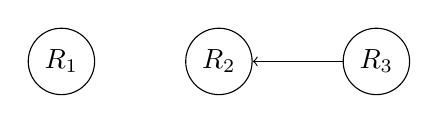
\begin{tikzpicture}[node distance=3cm]
\node[draw,circle] (11) at (-2,0) {$R_1$};
\node[draw,circle] (02) at (0,0) {$R_2$};
\node[draw,circle] (22) at (2,0) {$R_3$};
\draw[->] (22) -- (02);
\end{tikzpicture}
\end{center}
\vspace{-.4cm}
\caption{Example of a bidirectional utility diagram over three attributes. \label{fig:biut}}
\end{figure}

\citet{Abbas2010} identifies classes of bidirectional utility diagrams which give rise to optimal expansions of the multiattribute utility function, i.e. those where the conditional utility functions include the lowest number of arguments. 

For the purpose of this thesis we consider only a subclass of bidirectional utility diagrams. This was defined in \citet{Leonelli2015}.
 
\begin{definition}
\label{def:dirutdia}
We say that a bidirectional utility diagram is a \emph{directional utility diagram} if its graph is a DAG.
\end{definition}
Note that the diagram in Figure \ref{fig:biut} is unconventional in the sense that an attribute is parent of another one having a lower index. We  motivate this choice in Chapter \ref{chapter4}, where such diagrams proves to be very useful. Directional utility diagrams are extremely powerful in the multi-expert domains we address in later chapters, since the utility function associated to such diagrams can be written in terms of criterion weights and univariate utility functions. This is formalised in the following lemma.
\begin{lemma}
\label{lemma:ut}
For a directional utility diagram with vertex set $\{R_i:i\in[m]\}$ there exists an expansion order such that equation  (\ref{eq:genut}) is a linear combination of terms involving only criterion weights and conditional utility/disutility function having as argument a single attribute. 
\end{lemma}
\begin{proof}
This result follows by observing that the terms $u(\bm{r}_A^{0*},\bm{r}_{[m]\setminus A})$ in equation (\ref{eq:genut}) coincide with $u(\bm{r}_{[m]}^{0*})$ since the expansion can be performed over all the attributes. These terms are functions of criterion weights. Furthermore the conditional independence structure underlying a directed utility diagram is such that there is an expansion order where $R_i$ UI $\bm{R}_{V_i}\;|\; \bm{R}_{[m]\setminus \{V_i\cup i\}}$. Thus $g(r_i\;|\; \bm{r}_{B_i}^{0*},\bm{r}_{V_i})$ in equation (\ref{eq:genut}) is equal to $g(r_i\;|\; \bm{r}_{B_i}^{0*})$.
\end{proof}

\subsection{Univariate Utility Theory}
\label{sec:univariate}
In the previous sections we have shown how multiattribute utility problems can be decomposed into univariate ones when various sets of independences are believed to hold. We now discuss some of the characteristics of univariate utility functions and provide various examples. 

First, recall that utility functions are unique up to affine transformations, meaning that they imply the same preference ranking. Two such functions are said to be \textit{strategically equivalent}. In addition, \citet{Keeney1993a} showed that if two utility functions are strategically equivalent, then one must be an affine transformation of the other. 

We now introduce a variety of utility functions widely used in practice. 
\begin{example}
For the purpose of this example, we make explicit the dependence on the decision $\bm{d}$. Choices for $u_i(r_i,\bm{d})$ are 
\begin{itemize}
\item the \emph{linear utility} function, $u_i(r_i,\bm{d})= a(\bm{d})+b(\bm{d})r_i$, for $b(\bm{d})>0$;
\item the \emph{quadratic utility},  $u_{i}(\bm{d},r_{i} )=1-(\rho_{i}(\bm{d})r_{i})^{2}$, whose parameter is specified through the ideal scenario $\rho _{i}(d)$;
\item the \emph{polynomial utility} of degree $l$, $ u_i(\bm{d},r_i)=\sum_{j\in[l]}\rho_{ij}(\bm{d})r_i^j,$ where both the coefficients $\rho_{i,j}(\bm{d})$ and the domain of the rewards need to entertain some constraints \citep[see][for a discussion of these, which we omit here since are not relevant for our developments]{Keeney1993a,Muller1987};\footnote{Note that the polynomial utility has no monomial of degree zero. This is because many of the results of Chapter \ref{chapter5} are more easily interpretable in this case. Recall that adding such a monomial does not change the analysis as the two utilities are strategically equivalent.} 
\item the \emph{exponential utility} function, $
u_{i}(r_{i},\bm{d} )=1+\exp \left\{ -\rho _{i}(\bm{d})r_{i}\right\}$, where the parameter $\rho _{i}(\bm{d})>0$, reflects the degree of risk aversion.
\end{itemize}
\end{example}

Many of the characteristics of a univariate utility function, as for example whether it is monotonic and convex or not, describe the preferences of the DM and her attitude towards risk. See for more details on this \citet{Keeney1993a}.

\section{Graphical Decision Models}
\label{sec:dec}
In the previous sections we assumed the existence of a generic decision space $\bm{\mathcal{D}}$ representing the available choices to a DM. However, in practice, DMs have to commit to a sequence of decisions, where some of the consequences of committing to a certain action are observed before having to choose subsequent policies. Such a sequential structure can be depicted through graphical representations of various types. Here we focus on the Influence Diagram (ID) model, which can be thought of as an augmented version of a BN including also decision and utility vertices. 
These are introduced in Section \ref{sec:id}. We  note that, although widely used in practice, IDs are able to represent decision problems entertaining fierce symmetric conditions. In Section \ref{sec:asy} we provide a brief overview of the available models for the so called asymmetric decision problems.
 
For the purpose of this section, we slightly change our notation, which turns out to be very useful in concisely represent many of the features related to IDs. Furthermore, as shown in Section \ref{sec:symbolic}, this enables a straightforward implementation of the study of these models in a computer algebra system. This is a new representation of IDs that we introduced in \citet{Leonelli2015a}. Let $[n]$ be partitioned in $\mathbb{V}$ and $\mathbb{D}$, where $\mathbb{V}$ is the index set of the random (or non-controlled) variables, whilst $\mathbb{D}$ is the index set of the decisions (or controlled variables). 

\begin{example}
Let $n=6$ and assume $\mathbb{D}=\{1,4\}$ and $\mathbb{V}=\{2,3,5,6\}$. Then $Y_1$ and $Y_4$ are decisions, whilst $Y_2$, $Y_3$, $Y_5$ and $Y_6$ are random variables. 
\end{example}

\subsection{Influence Diagrams}
\label{sec:id}
As noted above, only decision problems enjoying strong symmetry conditions can be represented as IDs \citep{Howard1983,Howard2005a, Jensen2009, Shachter1986,Shachter1989a,Smith2010}. We define here, following \citep{Smith2008e,Smith2010}, the class of problems that entertains such a representation, that we call uniform.
\begin{definition}
\label{def:udp}
A  \emph{uniform decision problem} is such that:
\begin{itemize}
\item a variable $Y_i$, $i\in \mathbb{D}$, is controlled before controlling $Y_j$, $j\in \mathbb{D}$, if $i<j$, and is remembered when making decisions with a higher index;\footnote{With the term \textit{controlled} we mean that a decision variable is implemented.}
\item the space $\bm{\mathcal{Y}}_{[n]}$ is the product of the individual spaces, i.e. $\bm{\mathcal{Y}}_{[n]}=\bigtimes_{i\in[n]}\mathcal{Y}_i$;
\item if a random variable $Y_i$, $i\in\mathbb{V}$, is observed before a variable $Y_j$, then $i<j$ and its distribution can depend  on $\bm{Y}_\mathbb{D}$ only through $\bm{Y}_{\mathbb{D}\cap[i{-1}]}$.
\end{itemize}
\end{definition}
The condition in the first bullet is usually referred to as no-forgetting. This bullet further implies that decisions are totally ordered. Furthermore decisions and random variables cannot be constrained with each other in uniform decision problems, as specified by the second bullet. The third bullet corresponds to the causal consistency lemma of \citet{Cowell1999a} and guarantees that decisions cannot influence variables that have been already observed.

As briefly mentioned, the vertex set of an ID consists of random variables, decisions and utilities. We focus now on the latter type of nodes. The ID literature usually assumes that there is an additive factorisation between the utilities associated to different vertices. We refer to such IDs as \textit{additive IDs}. In \citet{Leonelli2015a} we defined the \textbf{Multiplicative Influence Diagram (MID)} which considers  the much larger class of multiplicative utility factorisations.  Let $\mathbb{U}=\{u_i:i\in[m]\}$ and $u_i$, $i\in[m]$, maps a subspace $\bm{\mathcal{Y}}_{P_i}$ of $\bm{\mathcal{Y}}_{[n]}$ into $[0,1]$, with $P_i\subseteq [n]$.

\begin{definition}
\label{def:MID}
An  \emph{MID} $\Gr$  consists of
\begin{itemize}
\item a DAG with vertex set $V(\Gr)=\{Y_i,u_j: i\in[n], j\in[m]\}$ and edge set $E(\Gr)$ including three types of edges defined by the following rules:
\begin{itemize}
\item for $i\in [m]$, $u_i$ has no children. Its parent set is $\{Y_j: j\in P_i\}$ and an index $i\in[n]$ can appear in a set $P_j$ only, $j\in[m]$, i.e. an element of $\{Y_i:i\in[n]\}$ is parent of at most one element of $\mathbb{U}$. For $u_i$ and $u_j$, $i,j\in[m]$, $i>j$ if there is a $k\in P_i$ such that for every $l\in P_j$, $k>l$: i.e. a utility node $u_i$ has higher index than $u_j$ if one parent of $u_i$ has higher index than all parents of $u_j$;
\item for $i\in\mathbb{D}$, the parent set of $Y_i$, $\{Y_j: j\in \Pi_i\}$, for $\Pi_i\subset[n]$, consists of the random variables and the decisions that are known when $Y_i$ is controlled;
\item for $i\in \mathbb{V}$, the parent set of $Y_i$,  $\{Y_j: j\in \Pi_i\}$, for $\Pi_i\subset[n]$, is such that $
Y_i \independent  \bm{Y}^{i}_{[n]}\;|\;\bm{Y}_{\Pi_i},\bm{\theta}$;
\end{itemize}
\item for $i\in\mathbb{V}$, a  density function $f_i(y_i\;|\;\bm{y}_{\Pi_i},\bm{\theta}_i)$; 
\item a multiplicative utility factorisation over $\mathbb{U}$.
\end{itemize}
\end{definition} 

Therefore, in an MID there are three types of vertices and three types of edges. The vertices are either random variables, decisions or utilities. Random variables are framed in circles, decisions in squares, whilst utilities have no framing in the DAG $\Gr$ of an MID. An edge into a vertex associated to a random variable asserts that the density of that random variable is conditional on the variable associated to the parent vertex. This edge therefore represents probabilistic dependence. Edges into decision vertices are called \textit{information} edges. These imply that the variables in the parent vertex are known when making that decision. Edges into utility vertices simply represent functional relationships, meaning that the utility is a function of the parent variables. \citet{Smith2010} defined the reduced ID, where some of the information edges are not included, thus rendering the overall graphical representation clearer. Specifically, in a reduced ID no edge $(Y_k,Y_i)$ is included if $(Y_k,Y_j)\in E(\Gr)$, $k<j<i$, $j,i\in\mathbb{D}$. 

 IDs are extremely powerful graphical representations of the qualitative structure underlying the elements of decision problems. In particular, these are able to depict both continuous and discrete domains. Note that although $P_i$, $i\in [m]$, is effectively an index parent set, we had to use a different notation than the one generically introduced for graphs in Appendix $\ref{appendixB}$, because of the existence of both utility and non-utility nodes.

Definition \ref{def:MID} implies a total order over the vertex set of an MID. For $i\in[m]$, let $j_i$ be the highest index of $P_i$ and $\mathbb{J}=\{j_i:i\in[m]\}$. The totally ordered sequence associated to $V(\Gr)$ is called \textbf{Decision Sequence (DS)} of the MID $\Gr$ and  indicated as   $S:=(Y_1,\dots,Y_{j_1},u_1,Y_{j_1+1},\dots,Y_{j_m},u_m)$.  In contrast with other authors \citep[e.g.][]{Jensen2009,Cowell1999a}, we do not introduce utility nodes only at the end of the DS. This entails an efficient computation of the expected utility scores, since optimal decisions can be shown to be functions of smaller sets of preceding variables.

\begin{example}
Figure \ref{fig-ex} presents an MID with vertex set $\{Y_1,\dots, Y_6, u_1,\dots, u_3\}$ describing a gross simplification of the possible countermeasures after an accident at a nuclear power plant. For this MID, $n=6$, $m=3$, $\mathbb{D}=\{1,4\}$ and $\mathbb{V}=\{2,3,5,6\}$. Therefore, there are two decisions $Y_1$ and $Y_4$: the first consisting of the possibility of closing down the power plant, the second of evacuating the nearby population. Before controlling $Y_4$, the variables $Y_1$, $Y_2$ and $Y_3$ are observed since $\Pi_4=\{1,2,3\}$.
 There are four random nodes: $Y_2$ and $Y_3$ measure the amount of dispersion of the contaminant in the atmosphere and to the ground respectively, $Y_5$ estimates the human intake of radiation and $Y_6$ ranks the level of stress in the population. This DAG implies for example that $Y_5\independent Y_2\;|\;Y_3$ for every $y_1\in\mathcal{Y}_1$ and $y_4\in\mathcal{Y}_4$. The variable $Y_5$ has parent set $\{Y_3, Y_4\}$,  $\Pi_5=\{3,4\}$ and $\Pi_{5\cap\mathbb{V}}=\{3\}$. We further assume all  variables to be binary, taking values in the spaces $\mathcal{Y}_i=[1]^0$, $i\in [6]$. When $\mathcal{Y}_i$ is associated to a decision node, 1 and 0 correspond to, respectively, proceed and not proceed. If  $\mathcal{Y}_i$ is associated to a random node, then 1 and 0 correspond respectively to high and low.
  The MID definition is completed by three utility nodes, $u_1$, $u_2$ and $u_3$. For example the set $P_3$ is equal to $\{4,6\}$ and therefore $Y_4$ and $Y_6$ are the arguments of the utility function $u_3$. Lastly, the  DS $(Y_1,Y_2,Y_3,u_1,Y_4,Y_5,u_2,Y_6,u_3)$ is the one associated to the MID in Figure \ref{fig-ex}, where $j_1=3$, $j_2=5$, $j_3=6$ and $\mathbb{J}=\{3,5,6\}$.  
\end{example}

\begin{figure}
\vspace{0.4cm}
\centerline{
\xymatrix{
*+[F]{Y_1}\ar@/^2pc/[rr]\ar[r]\ar[rd]&*+[Fo]{Y_3}\ar[dl]\ar@/^2pc/[rr]\ar[r]&*+[F]{Y_4}\ar[d]\ar[r]\ar[rd]&*+[Fo]{Y_5}\ar[r]\ar[d]&u_2\\
u_1&*+[Fo]{Y_2}\ar[u]\ar[ru]&u_3&*+[Fo]{Y_6}\ar[l]&
}
}
\vspace{0.2cm}
\caption{An influence diagram describing the available countermeasures after an accident at a nuclear power plant.}
\label{fig-ex}
\end{figure}

The density associated to an MID enjoys a factorisation which mirrors the one of BNs.

\begin{proposition}
\label{lemma:id}
The probability density function associated to an MID can be written as
$
f(\bm{y}_{\mathbb{V}}\;|\;\bm{\theta})=\prod_{i\in{\mathbb{V}}}f(y_i\;|\;\bm{y}_{\Pi_i},\bm{\theta}_i),
$
where $\bm{\theta}^\T=(\bm{\theta}_i)_{i\in\mathbb{V}}$.
\end{proposition}

\begin{example}
The density function associated to the MID in Figure \ref{fig-ex} can be written as
\begin{equation*}
f(\bm{y}\;|\;\bm{\theta})=f(y_2\;|\;y_1,\bm{\theta}_2)f(y_3\;|\;y_2,y_1,\bm{\theta}_3)f(y_5\;|\;y_4,y_3,\bm{\theta}_5)f(y_6\;|\;y_5,y_4,\bm{\theta}_6).
\end{equation*}
The utility factorisation associated to this MID coincides with the one in equation (\ref{eq:examplemultilinear})
\end{example}
\subsubsection{The Evaluation of Influence Diagrams.} 
To \textit{evaluate} an MID is to identify a sequence of optimal decisions maximising the expected utility function. However, only  MIDs whose topology is such that, for any index $j\in\mathbb{D}$, the only variables that are known at the time the DM makes a decision $Y_j$  have an index lower than $j$, can be directly evaluated using standard \lq{e}xtensive form'   calculations \citep{Smith1989a}. This is because the evaluation outputs optimal decisions as functions of observed quantities only and therefore DMs can unambiguously commit to such an optimal course of action. Here we define this class using the terminology of \cite{Smith2010}.
\begin{definition}
\label{ei}
An MID $\Gr$  is in \emph{extensive form} if $i\in\Pi_j$, for all $j\in\mathbb{D}$ and $i\in[j{-1}]$. 
\end{definition}
We assume here for the sake of simplicity that the MID under study is in extensive form. However, we note here that any MID in non extensive form can be transformed into one that is: albeit sometimes with the loss of some efficiency. There are several rules, which we do not introduce here, to manipulate the topology of an MID, as for example, edge reversal and barren node removal \citep[see e.g.][]{Jensen2009,Shachter1986}, such that the resulting MID is in extensive form.  Without restriction we also assume that every vertex $Y_i$ of the MID, $i\in [n]$, has at least one child. Random and controlled vertices with no children could be simply deleted from the graph without changing the outcome of the evaluation of the MID \citep[see e.g.][]{Jensen2009}.  

\begin{example}
The MID in Figure \ref{fig-ex} is in extensive form since $\Pi_4=\{1,2,3\}$. If either the edge $(Y_2,Y_4)$ or $(Y_3,Y_4)$ were deleted from this diagram, then the MID would not be in extensive form any more. Furthermore note that the only vertices with no children are $u_1$, $u_2$ and $u_3$. 
\end{example}

Several algorithms have now been defined to evaluate IDs. These can work directly on the ID \citep{Shachter1986,Olmsted1983}, transform it into a decision tree \citep{Canbolat2007}, or convert the diagram into some other graphical structure \citep{Jensen1994,Madsen1999}. There were severe computational issues related to the evaluation of IDs, but there are now several  promising methodologies designed to overcome these challenges, as noted in \citet{Bielza2011} and \citet{Gomez2007}. Many different pieces of software are also now available to build and automatically evaluate large IDs \citep{Jensen2013}. The simplest way to evaluate an MID in extensive form is through a backward inductive algorithm over the vertices of the DAG \citep[see e.g.][]{Jensen2009}. Here we introduce a computationally efficient new version of this algorithm, including at each step only the strictly necessary utility nodes. For simplicity, we work with the predictive distribution $f(\bm{y})=\int_{\bm{\Theta}}f(\bm{y}\;|\;\bm{\theta})f(\bm{\theta})$, but the result can be straightforwardly generalised to take into account the parameter vector.  The identification of the optimal policy is based on the computation of the functions $\bar{u}_i(\bm{y}_{B_i})$, $i\in[n]$, we formally introduce in Proposition \ref{i-th}, where 
\begin{equation}
\label{Ai}
B_i=\left\{\bigcup_{k\in[n]_{i-1}\cap\mathbb{V}}\Pi_k\;\;\;\;\bigcup\bigcup_{j\in[n]_{i-1}\cap \mathbb{J}}P_j\right\}\setminus[n]_{i-1},
\end{equation}
is the index set of the variables that appear as arguments of $\bar{u}_i$, where $[n]_{i-1}=\{i,\dots,n\}$. It should be noted that $B_i$ includes only indices smaller than $i$ that are either in the parent set of a random variable $Y_k$, $k>i$, or in a set $P_j$ such that $u_j$ succeeds $Y_i$ in the DS of the MID.

\begin{example}
We compute here the sets $B_5$ and $B_4$ associated with the MID in Figure \ref{fig-ex}. The set $B_5=\{3,4\}$ since $B_5=\{\Pi_6\cup \Pi_5\cup P_3\cup P_2\}\setminus\{5,6\}$, where $\Pi_6=\{4,5\}$, $\Pi_5=\{3,4\}$, $P_3=\{4,6\}$ and $P_2=\{5\}$. Furthermore $B_4=\{3\}$ since it can be noted that $B_4=B_5\setminus \{4\}$.
\end{example}

\begin{proposition}
\label{i-th}
The optimal decision associated to an MID yields expected utility $\bar{u}_1(\bm{y}_{B_1})$, where, for $i\in[n]$, $\bar{u}_i(\bm{y}_{B_i})$ is defined as
\begin{equation*}
\label{eq:id1}
\bar{u}_i(\bm{y}_{B_i})=\left\{
\begin{array}{lcl}
\bar{u}_i^{\mathbb{D}}(\bm{y}_{B_i}),&&\mbox{if } i\in\mathbb{D},\\
\bar{u}_i^{\mathbb{V}}(\bm{y}_{B_i}),&&\mbox{if } i\in\mathbb{V},
\end{array}
\right.
\end{equation*}
where, for $i=n$,
\begin{align}
&\bar{u}_n^{\mathbb{D}}(\bm{y}_{B_n})=\max_{\mathcal{Y}_n}k_mu_m(\bm{y}_{P_m}),\hspace{1cm }\bar{u}_n^{\mathbb{V}}(\bm{y}_{B_n})=\int_{\mathcal{Y}_n}k_mu_m(\bm{y}_{P_m})f_n(y_n\;|\;\bm{y}_{\Pi_n})\dr y_n,\label{cond4}\\
\intertext{and, for $i\in[n-1]$, if $i\in \mathbb{J}$ and supposing $i\in P_l$,}
&\bar{u}_i^{\mathbb{D}}(\bm{y}_{B_i})=\max_{\mathcal{Y}_i}\Big(hk_lu_l(\bm{y}_{P_l})\bar{u}_{i+1}(\bm{y}_{B_{i+1}})+k_lu_l(\bm{y}_{P_l})+\bar{u}_{i+1}(\bm{y}_{B_{i+1}})\Big),\label{cond2}\\
&\bar{u}_i^{\mathbb{V}}(\bm{y}_{B_i})=\int_{\mathcal{Y}_i}\hspace{-0.15cm}\Big(hk_lu_l(\bm{y}_{P_l})\bar{u}_{i{+1}}(\bm{y}_{B_{i{+1}}})+k_lu_l(\bm{y}_{P_l})+\bar{u}_{i{+1}}(\bm{y}_{B_{i{+1}}})\Big)f_i(y_i\;|\;\bm{y}_{\Pi_i})\dr y_i\label{cond3},\\
\intertext{whilst, if $i\not\in\mathbb{J}$,}
&\bar{u}_i^{\mathbb{D}}(\bm{y}_{B_i})=\max_{\mathcal{Y}_i}\bar{u}_{i+1}(\bm{y}_{B_{i+1}}),\hspace{1cm}\bar{u}_i^{\mathbb{V}}(\bm{y}_{B_i})=\int_{\mathcal{Y}_i}\bar{u}_{i+1}(\bm{y}_{B_{i+1}})f_i(y_i\;|\;\bm{y}_{\Pi_i})\dr y_n.\label{cond1}
\end{align}
\end{proposition}
The proof of this result is given in Appendix \ref{appendixA1}. In Section \ref{sec:symbolic} we symbolically define MIDs and introduce a new symbolic evaluation algorithm.

\subsection{Asymmetric Models}
 \label{sec:asy}
The ID framework is able to represent uniform decision problems only. However, real decision problems often exhibit asymmetries of various kinds. In \citet{Jensen2009} asymmetries are categorised in three classes. If the possible outcomes or decision options of a variable vary depending on the past, the asymmetry is called \textit{functional}. If the very occurrence of a variable depends on the past, the asymmetry is said to be \textit{structural}. \textit{Order} asymmetries are present if $\{Y_i:i\in\mathbb{D}\}$ is not totally ordered. We note here that there are four types of functional asymmetries that can occur:
\begin{itemize}
\item \textbf{chance} $\rightarrow$ \textbf{chance}: the outcome of random variables restricts the outcomes of other random variables;
\item \textbf{chance} $\rightarrow$ \textbf{decision}: the outcome of random variables restricts the options of controlled variables;
\item \textbf{decision} $\rightarrow$ \textbf{chance}: decisions taken restrict the possible outcomes of random variables;
\item \textbf{decision} $\rightarrow$ \textbf{decision}:  decisions taken restrict the options of other controlled variables.
\end{itemize}
Heuristically, for each of these asymmetries the observation of $\bm{y}_A$, $A\subset [n]$, changes the space $\bm{\mathcal{Y}}_B$ associated to a vector $\bm{Y}_B$, such that $A\cap B=\emptyset$. This new space, $\bm{\mathcal{Y}}_B'$ say, is a subspace of $\bm{\mathcal{Y}}_B$.

The simplest solution to the evaluation of an asymmetric problem is by embedding it in a symmetric one which can be represented as an ID. The above mentioned evaluation algorithms can then be used to identify optimal solutions in the embedded version of the problem. Clearly this methodology has several drawbacks. Most importantly it does not graphically represent the relevant asymmetries and often considers a much larger problem space than the original one. For this reason a variety of graphical models have been introduced to represent a variety of asymmetric constraints \citep{Smith1993,  Demirer2006a, Nielsen2003, Jensen2006, Jensen2002, Bhattacharjya2012}. It is not the purpose of this thesis to review these models and we briefly illustrate part of the semantic of the sequential ID \citep{Jensen2006} model in the following example. 

\begin{example}
\label{eee}
Consider the ID in Figure \ref{fig-ex} and assume that the DM now believes her decision problem is characterised by the following three asymmetries:
\begin{itemize}
\item whenever she decides to close the power source, then the population cannot be evacuated from the area: $Y_1=1\Rightarrow Y_4=0$;
\item if either the deposition or the dispersion levels in the area are high, then  the human intake is high: $Y_2=1 \lor Y_3=1\Rightarrow Y_5=1$;
\item if the evacuation option is followed then both the human intake and the stress levels in the population are high: $Y_4=1\Rightarrow Y_5=1 \land Y_6=1$.
\end{itemize}
\end{example} 
\begin{figure} 
\vspace{-0.3cm}
\begin{center}
\begin{tikzpicture}[node distance=4cm]
\node[draw,rectangle] (00) at (0,0) {$Y_1$};
\node[draw,circle] (1-1) at (2,-1) {$Y_3$};
\node[draw,circle] (11) at (2,1) {$Y_2$};
\node[draw,rectangle] (20) at (4,0) {$Y_4$};
\node[draw,circle] (31) at (8,1) {$Y_6$};
\node[draw,circle] (3-1) at (8,-1) {$Y_5$};
\node (0-1) at (0,-1) {$U_1$};
\node (21) at (4,1) {$U_3$};
\node (4-1) at (10,-1) {$U_2$};
\draw[->] (00) -- (11);
\draw[->] (00) -- (1-1);
\draw[->,anchor=center, below] ([yshift=0.1cm]00.east) to node {} ([yshift=0.1cm]20.west);
\draw[->,dashed,anchor=center, below] ([yshift=-0.1cm]00.east) to node {\tiny{$Y_1=4|Y_4=0$}} ([yshift=-0.1cm]20.west);
\draw[->] (11) -- (1-1);
\draw[->] (1-1) -- (0-1);
\draw[->] (20) -- (21);
\draw[->] (31) -- (21);
\draw[->] (3-1) -- (4-1);
\draw[->] (11) -- (20);
\draw[->] (1-1) -- (20);
\draw[->] (1-1) -- (3-1);
\draw[->,anchor=center, below] (20.north) to node {} (31);
\draw[->,anchor=center, below] (20.south) to node {} (3-1);
\draw[->] (3-1) -- (31);
\node[draw=black, dashed, ellipse, inner sep =4pt, fit= (11) (1-1)] (circ1) {};
\node[draw=black, dashed, ellipse, inner sep =4pt, fit= (31) (3-1)] (circ2) {};
\draw[->, dashed,anchor=center, below] ([yshift=-1.2cm]circ1.east) to node {\tiny{$Y_2=1,Y_3=1|Y_5=1$}} ([yshift=-0.2cm]3-1.west);
\draw[->, dashed,anchor=center, above] (20) to node {\tiny{$Y_4=1|Y_5=1,Y_6=1$}} (circ2.west);
\end{tikzpicture}
\end{center}
\vspace{-0.4cm}
\caption{Representation of the asymmetric version of the multiplicative influence diagram of Figure \ref{fig-ex} as a sequential influence diagram. }\label{sid}
\end{figure}

Our graphical representation of these asymmetries is given in Figure \ref{sid}, corresponding to a sequential ID \citep{Jensen2006}. Asymmetries are represented as labels on additional dashed arcs. If the asymmetry is composite, meaning that it involves more than two variables, then vertices can be grouped through a dashed ellipse and dashed arcs can either start or finish by the side of these ellipses. As exemplified by the diagram in Figure \ref{sid}, the graphical representation of asymmetric decision problems, although providing a framework to quickly identify optimal policies, often lose the intuitiveness and the clarity of representation of standard IDs. We discuss more extensively this issue in Section \ref{sec:symbolic}. 

Asymmetric decision problems can also be explicitly modelled as \textit{decision trees} \citep[see e.g.][]{Clemen1996a,French2009}, an augmented version of an event tree including decision vertices and whose leaves are utilities. These suffer the same drawbacks of staged and event trees. Recently \citet{Cowell2010} introduced the decision CEG which can more compactly represent asymmetric decision problems.
 
\section{Group Decision Making}
\label{sec:group}
The SEU model characterises rational decision making for single DMs. However, in practice, most decisions in organisations and society are the responsibility of groups rather than individuals: juries, cabinets and boards of directors are some examples. In addition, even single DMs rarely commit to certain courses of actions without seeking for the help of appropriate experts. How the suggestions of various experts have to be reconciled is a very interesting question and a variety of solutions have been proposed. Following \citet{French2011}, we identify two main contexts of group decision making:
\begin{itemize}
\item the \textbf{group decision problem}: a group of individuals is jointly responsible and accountable for the decision;
\item the \textbf{expert problem}: a group of experts are consulted by a single DM who is responsible and accountable for the decision to be made.
\end{itemize}
\citet{French2011} also identifies the \textit{textbook problem} context which for the purpose of this thesis is not discussed here. Note further that a combination of the two above scenario can be considered in practice. There are two main categories of approaches for both contexts: behavioural and mathematical. We review the former ones in Section \ref{sec:decconf}.

Mathematical approaches for the group decision problem are based on some algorithmic rule which, given the preferences and beliefs of each individual DM, then outputs the decision ranking of the group. We do not focus in this thesis on these methods and we simply note here that there is vast literature about these \citep[see e.g.][]{Arrow1963,Keeney1976, Keeney1993a, French2009,French2011,Keeney2013}. Most of these methods, embedding some idea of democratic voting, are subject to paradoxes and inconsistencies. We discuss mathematical approaches for the expert problem in Section \ref{sec:expert}.
 
\subsection{Behavioural Approaches}
\label{sec:decconf}

\textit{Decision conferences} and \textit{facilitated workshops} are the most common techniques of behavioural aggregation of DMs' beliefs and preferences \citep{ Ackermann1996,Phillips1984,Phillips1993}. These are usually two days events with around fifteen participants \citep[although for example in the Chernobyl project we discussed in Chapter \ref{chapter1} the number of participants was way larger, as noted in][]{French2009}. In such meetings, a \textit{facilitator}, an individual skilled in the process of group discussion, encourages debate among the DMs and keeps the group's focus on the issue at hand. The facilitator is usually not an expert of the problem to be examined and has no ownership of the decision to be made. Each DM often has available interactive software to run her own analyses and observe the results of others' beliefs, which are also projected in the room. This software uses decision models which turns out to be fundamental to foster discussion and raise the main issues that need to be investigated by the group. The results of sensitivity analyses are also shown to the DMs in order to build consensus and avoid debates on irrelevant alternatives or parameters that do not affect the group's course of action. 

As discussed in Chapter \ref{chapter1}, these types of meetings were central to the decision elicitation process within the Chernobyl Project. The discussions at those meetings are summarised in \citet{French2009} and \citet{Smith2010}. \citet{Ackermann1996} reports more than 100 of successful applications of such behavioural techniques. 

A different method called \textit{Delphi protocol} has been designed to reach consensus by the remote and electronic compilation of a series of questionnaire, thus not requiring the group to meet \citep{Dalkey1963,Linstone1975}. Under this protocol, each individual anonymously responds to the questionnaire. The answers are then sent to the other members for further comments and generations of possible courses of actions. This sequence is then iteratively repeated until consensus is reached. 
 
\subsection{The Expert Problem}
\label{sec:expert}

The second context where groups are involved in the decision making process is the expert problem. Here an individual DM needs to synthesise the beliefs of a group of $m$ experts into a unique probability distribution. Mathematical methods for the aggregation of expert judgement can be broadly categorised into two main branches: Bayesian and pooling operator methods. Before discussing these approaches, we remark that it is not the scope of this thesis to explore the validity of each of these \citep[see e.g.][and the references therein for an extensive discussion]{Clemen99,French2011}. \citet{O'Hagan2006a} discussed protocols to be followed by each expert to elicit his own probability distribution, whilst \citet{Merrick2008} introduced methods to identify the right mix of experts to obtain the best aggregated belief. Here we mostly focus on pooling operators and we simply note that the Bayesian approach treats experts' judgements as data, synthesised in some appropriate likelihood function, to update the prior probability of the DM \citep[see e.g.][]{French1980, Mumpower1996,Wiper1995c,Albert2012}.

\subsubsection{Pooling Operators.}
\label{sec:pool}
Given the individual probabilities of a group of $m$ experts, $f^i(\bm{y})$, $i\in[m]$, pooling operators consist of a function  $T^p$ which pools together into a unique probability distribution, $f^{DM}(\bm{y})$, the probability distributions of each member of the group. For ease of notation we suppress the dependence on the parameter vector.

The simplest operator is the \textit{linear} one \citep{Stone1961}, corresponding to a weighted average of the experts' distributions:
\begin{equation*}
\label{eq:linearpool}
f^{DM}(\bm{y})=\T^p(f^1(\bm{y}),\dots, f^m(\bm{y}))=\sum_{e\in[m]} w^ef^e(\bm{y}).
\end{equation*} 
\citet{Bacharach1975} introduced the \textit{logarithmic Operator (logOp)} defined as
\begin{equation*}
\label{eq:logpool}
f^{DM}(\bm{y})=\T^p(f^1(\bm{y}),\dots, f^m(\bm{y}))\propto\prod_{e\in[m]}f^e(\bm{y})^{w^e}.
\end{equation*}

One of the main issues concerning pooling operators is the identification of the weights $w_e$ to be given to each expert. The aggregation most commonly used in practice is through a linear operator whose weights are calibrated according to the forecasting performance of the experts on a calibration set of uncertain quantities. This method is usually called \textit{classical} approach to the combination of expert judgements \citep{Cooke1991a}.

Sets of axioms characterising operators encoding rational behaviour have been defined \citep[see for a review][]{Genest86}.  We argue here, following \citet{Faria1997}, that one very desirable property for a pooling operator is to be \textit{Externally Bayesian (EB)} \citep{Madansky64}. 
\begin{definition}
A pooling operator $\T^p$ is said to be EB if  $f^{DM}(\bm{y})$ is the same when the following two procedures are implemented:
\begin{itemize}
\item first apply $\T^p$ and then update $f^{DM}(\bm{y})$ using Bayes theorem;
\item first update each expert's distribution $f^i(\bm{y})$ via Bayes Theorem and then apply $\T^p$. 
\end{itemize}
\end{definition} 
Therefore for EB operators the order in which pooling and updating are performed is irrelevant. This is a desirable property for a variety of reasons: first, experts do not need to meet every time data is collected; second, experts cannot increase their influence on the outcome by choosing whether to include their beliefs before or after the collection of data; lastly, as we discuss below, operators exhibiting such a property are in general  able to retain the conditional independences underlying an agreed model.  Importantly, \citet{Genest84} characterised the logOp as the only operator being EB.
Although EB operators have useful properties in the domains we are addressing, we note that these operators have been criticised in the literature \citep[see e.g.][]{Lindley1985}.

\subsubsection{The Multivariate Case.}
When experts have to elicit probabilities in large multivariate settings, their performance might dramatically decrease because of the difficulty in assessing correlations \citep{Clemen2000,Winkler2004}. One approach often used to mitigate such difficulties is to elicit probabilities over an agreed qualitative graphical structure, as for example a BN \citep{Burns1993, Faria1997, Farr2015, Renooij2001,Smith2000}. \citet{Smith1996a} extensively argued that experts' agreement can be more easily found in graphical frameworks since the underlying conditional independence structure can be discussed in natural language.

 \citet{Pennock2005} proved that a pooled distribution obtained with a logOp reflects any shared Markov independence by the group and for this reason, it can be represented in a concise and natural manner with a BN as well. However, it was also noted that no pooling operator can maintain all independences representable in a BN. Having acknowledged this negative result, in Chapter \ref{chapter3} we develop a framework where groups of experts qualitatively agree on a specific graphical model and then quantitatively individually deliver probability judgements, preserving the group's conditional independence structure. 
 
 Here we focus on the work of \citet{Faria1996} and \citet{Faria1997} which assumes the presence of an underlying decomposable CG agreed by all the experts. Their work, introducing a generalisation of the logOp, falls within the pooling operators approach. Suppose the decomposable CG $\Gr$ has $n$ chain components $\{\bm{Y}_i:i\in[n]\}$ .
 
\begin{definition}
For a decomposable CG $\Gr$, the \textbf{conditional logOp}, $\T^P$, is defined by the components $\T^p_{\Pi_j}$ 
\begin{equation*}
\label{eq:clogop}
f^{DM}_j(\bm{y}_j\;|\;\bm{y}_{\Pi_j})=\T^p_{\Pi_j}(\cdot)\propto \prod_{i\in[m]}f_{j}^i(\bm{y}_j\;|\; \bm{y}_{\Pi_j})^{w_{j}^i(\Pi_j)},
\end{equation*}
where $f_{j}^i$ is is the conditional density relative to $\bm{Y}_j$ provided by the $i$-th expert and $w_{j}^i(\Pi_j)$ is a weight. The DM distribution is then defined as
\begin{equation*}
f^{DM}(\bm{y})=\T^p=\prod_{j\in[n]}\T^p_{\Pi_j}=\prod_{j\in[n]}  f^{DM}_j(\bm{y}_j\;|\;\bm{y}_{\Pi_j}).
\end{equation*}
\end{definition}

Although the conditional logOp is not EB, \citet{Faria1997} showed that it respects a weaker condition called Conditional External Bayesianity (CEB). 

\begin{definition}
Given a CG $\Gr$, \textbf{CEB} holds if the conditional densities $f_{j}^i(\bm{y}_j\;|\; \bm{y}_{\Pi_j})$, $i\in[m]$, $j\in[n]$, are pooled with an EB operator.
\end{definition}

We define here a class of likelihood functions that guarantees CEB when the pooling is performed with a conditional logOp.

\begin{definition}
\label{def:cutting}
A likelihood $l(\bm{x}\;|\;\bm{y})$ for a sample $\bm{x}^\T=(\bm{x}_i)_{i\in[n]}$ is in the class of \emph{cutting} likelihoods of a CG $\Gr$ with chain components $\{\bm{Y}_i:i\in[n]\}$ if
\begin{equation}
l(\bm{x}\;|\;\bm{y})=l_1(\bm{x}_1\;|\;\bm{y}_1)l_2(\bm{x}_2|\bm{y}_2, \bm{y}_{\Pi_2},\bm{x}_1)\cdots l_n(\bm{x}_n\;|\;\bm{y}_n,\bm{y}_{\Pi_n},\bm{x}^{n-1}).
\label{eq:cutting}
\end{equation}
\end{definition} 

\citet{Faria1997} then proved that the conditional logOp respects CEB when the pooling/updating is performed according to a procedure we briefly review here. Let $\tilde{f}_g$ be the joint density over $\Gr$ obtained by first pooling the individual posterior densities on $\bm{Y}_n\;|\; \bm{Y}_{\Pi_n}, \bm{X}$, then using the derived density on $\bm{X}\;|\; \bm{Y}^{n-1}$ to pool the  individual posteriors on $\bm{Y}_{n-1}\;|\;\bm{Y}_{\Pi_{n-1}},\bm{X}$, and so on. Conversely, let $\bar{f}_g$ the joint density over $\Gr$ obtained by first pooling the individual prior densities on $\bm{Y}_{n}\;|\;\bm{Y}_{\Pi_n}$ and forming the group's posterior density of $\bm{Y}_n\;|\;\bm{Y}_{\Pi_n},\bm{X}$, then pooling the individual priors on $\bm{Y}_{n-1}\;|\;\bm{Y}_{\Pi_{n-1}}$ and forming the posterior on $\bm{Y}_{n-1}\;|\;\bm{Y}_{\Pi_{n-1}},\bm{X}$ using the density of $\bm{X}\;|\;\bm{Y}^{n-1}$, and so on. We say that when these procedures are followed, the densities are \textit{backward sequentially updated}. It is apparent that an operator respecting CEB is such that $\tilde{f}(\bm{y}\;|\; \bm{x})=\bar{f}(\bm{y}\;|\;\bm{x})$.

\begin{proposition}
\label{prop:ceb}
The conditional logOp respects CEB for a decomposable CG $\Gr$ when distributions $f_{i}^j(\cdot)$ and $f^{DM}_i(\cdot)$, $i\in[n]$, $j\in[m]$, are backward sequentially updated.
\end{proposition}
 
 In Chapter \ref{chapter3} we discuss a variation of this result to cases where different groups of experts are responsible for disjoint subsets of the vertices of the CG. Furthermore, in Chapter \ref{chapter4} we develop recursions in dynamic settings which mirror the backward 
sequential updating of \citet{Faria1997}. 

\subsubsection{Aggregation in Complex Problems.}
The previous sections considered situations where experts can simply provide probabilities, possibly in a multivariate setting, for the whole domain under study. However, as we have extensively argued, in the applications we have in mind this can be only rarely  the case. A first attempt to generalise such framework for expert judgement combination was proposed in \citet{Bordley2009}. In that paper each expert delivers probabilities over a separate, but related, set of events and aggregating methods are then developed to reconcile their judgements into a unique probability distribution.

In complex applications however, experts can rarely simply  deliver  numbers representing their estimates and the uncertainty around these. They often run their own models and observe their outputs to then deliver the required uncertainties \citep{French2011}. This should be apparent from the RODOS discussion in Chapter \ref{chapter1}. This issue was already noticed in nuclear emergency management in \citet{Cooke2000}. The ENSAMBLE project \citep{Krishnamurti2000,Mikkelsen2003} is another example of this type of combination, where the outputs of different meteorological models need to be combined into a unique weather forecast. These types of combinations introduce new challenges since correlated estimates and uncertainties may arise at both  the expert and the model level. 

\citet{French2011} pointed out that the issue becomes even more delicate when models need to be chained together as in the RODOS modules' structure exemplified in Figure \ref{networkino}. Very little has been said on this issue and some early discussion on possible solutions were proposed in \citet{French1991}.  In the following chapters we explicitly address these types of problems and define a framework to coherently network together models and expert judgements.
 
\section{Conclusions and Contributions}
This chapter has summarised the main aspects of the Bayesian approach to inference and decision making that are relevant for this thesis. We have reviewed a variety of methods to represent both the uncertainties and the preferences of individual DMs. However we have noted that current methods for groups of DMs and for combining the judgements of several experts in complex domains are limited. In the following chapters we extend  Bayesian methodology to allow for a coherent aggregation of experts' beliefs and preferences in complex domains. We are able to show that many of the graphical models we have introduced provide an intuitive basis to do this. 

Note that some of the concepts introduced in this chapter, namely directional utility diagrams, MIDs and their evaluation are original contributions to the literature. We discuss additional features of these models in the following chapters. 

\subsection{Contributions}
Having introduced in details the normative framework of Bayesian decision analysis and inference, we can now discuss more explicitly the contributions of this thesis to the literature. To increase readability, we discuss the extensions we propose in the same order as in the list on pages 13-14.
\begin{itemize}
\item in this chapter we have shown how probabilistic inference can be carried in a distributed fashion for a variety of models when certain independences are assumed for the model parameter vector (specified in Definition 2.3.9 for BNs, in Definition 2.3.21 for MNs, on page 39 for CEGs and in Proposition 2.3.39 for MDMs). In Section 3.6 we introduce weaker conditions for these models, enabling distributed inferences when different panels of experts deliver the required probabilities for disjoint subsets of the vertex set of the underlying graph;
\item  the combination rules for expert judgements of \citet{Faria1997} briefly reviewed in Proposition 2.6.5 work when each expert deliver probabilities for every variable of an underlying CG. We extend this result in Section 3.6 to cases where experts deliver judgements only for subsets of the graph's vertex set;
\item in Section 2.3.4 we introduced the Perlean notion of causality and discussed Perlean intervention in Definition 2.3.49. In Section 3.5 below we introduce a new notion of causality extending the one of Pearl in two ways: first, our definition does not require the existence of an idle system, but instead assumes the existence of a natural comparator - a decision rule which is standard in the domain examined;  second, it allows for more general interventions than the \lq{d}o\rq \;  standard operator;
\item Definition 2.4.23 introduced bidirectional utility diagrams, a flexible graphical representation of partial utility independence. In Chapter 4 (and specifically Definition 4.1.8 and Proposition 4.1.10) we introduce a particular subclass of these models and deduce the utility factorization associated to this subclass. Such a class, together with a few other assumptions often made in practice (see Section 4.1), we enables the distributed computation of expected utility $\bar{u}(\bm{d})$ of any policy $\bm{d}$ as discussed in Theorem 4.1.13;
\item the computation of the expected utilities for utilities in the class mentioned in the previous point  can be carried using a backward induction procedure which mirrors the routine of \citet{Faria1997} to pool probability distributions (explicated on page 72); in Chapter 4 we introduce new backward inductions that instead of pooling probability distributions, compute optimal expected utility in multi-expert domains; 
\item in Section 2.1.2 we introduced moments and discusses their role in summarizing the features of a distribution. \citet{Cowell1999a} and \citet{Nilsson2001} introduced closed form recursions to compute moments of additive factorizations, as the ones in Proposition 2.4.16, over a BN model. In Chapter 5 we generalize such recursions to compute moments for multilinear factorizations introduced in Proposition 2.4.11;
\item standard conditional independence, as discussed in Section 2.3.1., often implies separations between certain functions of the model's parameter that are not strictly required for the computation of the  moments mentioned in the point above. In Section 5.3 we introduce new separation conditions, often implied by conditional independence, allowing for the computations of the above moments;
\item we define new symbolic inferential techniques in CEG and ID models, extending current methods for discrete BNs. For these models, each entry of a probability table, $\theta_i$ say, is considered as an indeterminate of a polynomial (or equally as a variable in a computer algebra system) and inference is carried with no full numerical specification of the model's probabilities. For CEGs, we extend current methods from symmetric to asymmetric probabilistic models. For IDs, we introduce a symbolic definition of utility values and introduce the polynomial form of the expected utilities associated to these models.   
\end{itemize}